
\section{Choosing Inventory Policies}

\subsection{Variations on the EOQ model}
\label{sec:variations-eoq-model}

\begin{exercise}
  When choosing an inventory policy, i.e., a policy that decides when
  and how much to order, we need to understand the environment first
  in which the policy is going to operate. Can you use
  Exercise~\ref{ex:1} to come up with a characterization of the environment? 
  \begin{comment}
    A simple starting point is provided by this table.
    \begin{table}[h]
      \centering
    \begin{tabular}{l|l|l|l}
      Environment && &  \\ \hline
Demand & variability &deterministic/constant & Stochastic \\ 
& substitution effects & yes & no \\
\hline Supply & Lead time & $L=0$& $L>0$ \\ 
& perishable items & yes & no\\
& Joint ordering & yes & no\\
& Order size constraints &yes & no \\
\hline Cost structure &Ordering cost & $A=0$ & $A>0$ \\ 
& holding cost & $h=0$ &$h>0$ \\
& fixed backlog cost & $\pi=0$ &$\pi>0$\\
&variable backlog cost & $b=0$ &$b>0$\\
&lost sales cost &$k=0$ & $k>0$ \\
&quantity discounts &yes & no \\
\hline KPIs &fill rate $S$ & yes & no\\ 
& cycle service level &yes& no\\
    \end{tabular}
    \caption{(Incomplete) characterization of the environment of inventory policies}
      \label{tab:environment}
    \end{table}
  \end{comment}
\end{exercise}

\begin{exercise}
  Characterize the EOQ model by means of the table of the previous
  exercise.
  \begin{comment}
    \begin{table}[h]
      \centering
    \begin{tabular}{l|l|l|l}
      Environment && &  \\ \hline
Demand & variability &\boxed{deterministic/constant} & Stochastic \\ 
& substitution effects & yes & \boxed{no} \\
\hline Supply & Lead time & \boxed{$L=0$}& $L>0$ \\ 
& perishable items & yes & \boxed{no}\\
& Joint ordering & yes & \boxed{no}\\
& Order size constraints &yes & \boxed{no} \\
\hline Cost structure &Ordering cost & $A=0$ & $\boxed{A>0}$ \\ 
& holding cost & $h=0$ & $\boxed{h>0}$ \\
& fixed backlog cost & $\pi=0$ & $\boxed{\pi=\infty}$\\
&variable backlog cost & $b=0$ &$\boxed{b=\infty}$\\
&lost sales cost &$k=0$ & $\boxed{k=\infty}$ \\
&quantity discounts &yes & \boxed{no} \\
\hline KPIs &fill rate & $\boxed{S=1}$ & no\\ 
& cycle service level &yes& no\\
    \end{tabular}
    \caption{EOQ model }
      \label{tab:environment}
    \end{table}
  \end{comment}
\end{exercise}

\begin{exercise}
  In the next set of exercises we are going to modify the assumptions
  of the EOQ model with the aim to investigate how the environment
  affects the inventory policy. For the sake of comparison, sketch how the inventory behaves over time for the EOQ model and write down the cost function.

  \begin{comment}
\begin{center}
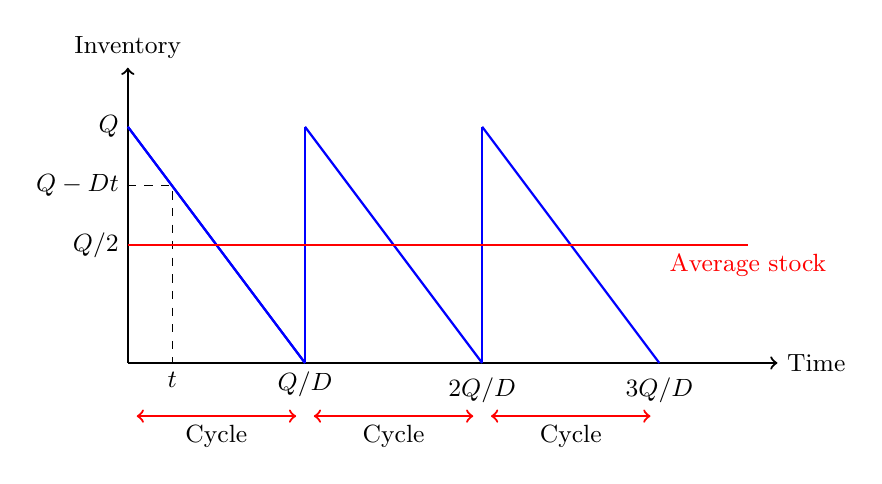
\begin{tikzpicture}[x=0.75cm,y=0.015cm]
\small
\draw[thick,->] (0,0) -- (11,0) node[right] {Time};
\draw[thick,->] (0,0) -- (0,250) node[above] {Inventory};
\draw[] (0,200) node[left] {$Q$};
\draw[color=blue,thick] (0,200) -- (3,0);
\draw[] (0.75,0) node[below] {$t$};
\draw[] (0,150) node[left] {$Q-Dt$};
\draw[dashed] (0,150) -- (0.75,150) -- (0.75,0);
\draw[] (3,0) node[below] {$Q / D$};
\foreach \y in {1,...,3}{
	\draw[color=blue,thick] (3*\y-3,200) -- (3*\y,0);}
\foreach \y in {1,2}{
	\draw[color=blue,thick] (3*\y,0) -- (3*\y,200);}
\foreach \y in {2,3}{
	\draw[] (3*\y,-5) node[below] {\y $Q/D$};}
\draw[] (0,100) node[left] {$Q / 2$};
\draw[color=red,thick] (0,100) -- (10.5,100) node[below] {Average stock};
\foreach \y in {0,...,2}{
	\draw[color=red,thick,<->] (3*\y+0.15,-45) -- (3*\y+3-0.15,-45);
	\draw[] (3*\y+1.5,-45) node[below] {Cycle};}
\end{tikzpicture}
\end{center}

The total cost for one cycle is the order cost plus the inventory cost. The order cost is $A$, the inventory cost is the total area of the triangle times $h$, i.e. 
\begin{equation*}
  \frac h2\text{height}\cdot\text{base} = \frac h 2 Q\cdot \frac QD= \frac h2 \frac{Q^2}D.
\end{equation*}
The average cost per unit time is this total cost divided by the duration of one cycle, which is $Q/D$. Therefore, the average cost is
\begin{equation*}
\frac A{Q/D}+  \frac{ h/2 \cdot Q^2/D}{Q/D} = \frac h 2 \frac {Q^2} D\cdot \frac D/Q = \frac D Q A + \frac h2 Q.
\end{equation*}

\begin{center}
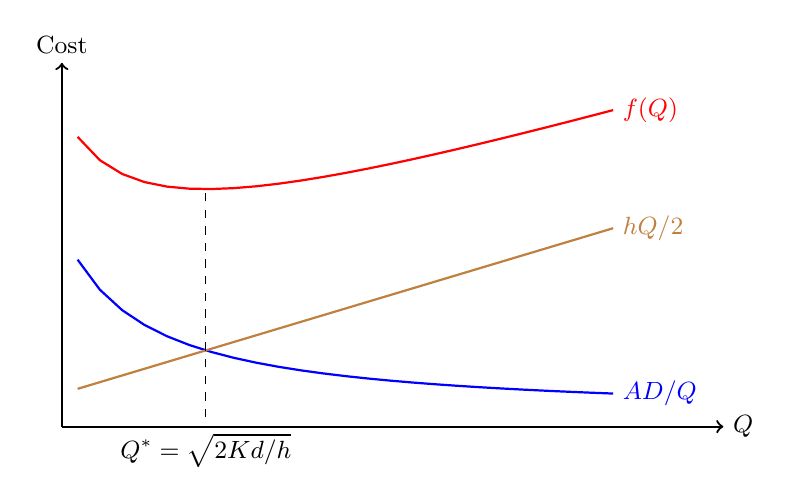
\begin{tikzpicture}[x=0.02cm,y=0.06cm]
\small
\def\c{1} 
\def\K{100} 
\def\h{0.2} 
\def\d{20} 
\pgfmathsetmacro{\Q}{sqrt(2)*sqrt(\K)*sqrt(\d)/sqrt(\h)}
\pgfmathsetmacro{\f}{sqrt(2)*sqrt(\K)*sqrt(\d)*sqrt(\h)+\c*\d}	
\draw[thick,->] (50,-2) -- (470,-2) node[right] {$Q$};
\draw[thick,->] (50,-2) -- (50,75) node[above] {Cost};
\draw[color=blue,thick,domain=60:400] plot (\x,{\d*\K/\x}) node[right] {$AD / Q$};
\draw[color=brown,thick,domain=60:400] plot (\x,{\h*\x/2}) node[right] {$hQ / 2$};
\draw[color=red,thick,domain=60:400] plot (\x,{\d*\K/\x+\c*\d+\h*\x/2}) node[right] {$f(Q)$};
\draw (\Q,-1.5) node[below] {$Q^{*} = \sqrt{2Kd / h}$};
\draw[dashed] (\Q,0) -- (\Q,\f);
\end{tikzpicture}
\end{center}

  \end{comment}
\end{exercise}

\begin{exercise}
  It is very important to memorize that the total inventory cost for
  the EOQ model is quite insensitive to the actual order quantity
  $Q$. Show this for the case with $A=100$, $h=0.2$, and $D=20$. What
  happens to the total cost if $Q=60, 80, \ldots 200$?
  \begin{comment}
From the EOQ formula
\begin{itemize}
\item $Q^{*} \approx 141.42$ units
\item $f(Q^{*}) \approx \mathdollar 48.28$
\end{itemize}

\begin{center}
\footnotesize
\begin{tabular}{rrrrr}
\toprule
$Q$     & $AD/Q$  &  $hQ/2$  & $f(Q)$ \\
\midrule
    60    & 33.33 &  6.00  & 59.33 \\
    80    & 25.00 &  8.00  & 53.00 \\
    100   & 20.00 &  10.00 & 50.00 \\
    120   & 16.67 &  12.00 & 48.67 \\
    140   & 14.29 &  14.00 & 48.29 \\
    160   & 12.50 &  16.00 & 48.50 \\
    180   & 11.11 &  18.00 & 49.11 \\
    200   & 10.00 &  20.00 & 50.00 \\
\bottomrule
\end{tabular}
\end{center}
  \end{comment}
\end{exercise}

\begin{exercise}
  As a first variation, what would you change/do if the lead time $L$
  is no longer 0, but becomes positive? (Thus, all the other
  assumptions of the EOQ model stay the same, only the lead time
  becomes positive.)  In other words, how would you change the EOQ
  policy, and determine when and how to order?
  \begin{comment}
    Since the backlog costs are infinite, backlogging is not
    desirable, hence we order early. See the graph: 
\begin{center}
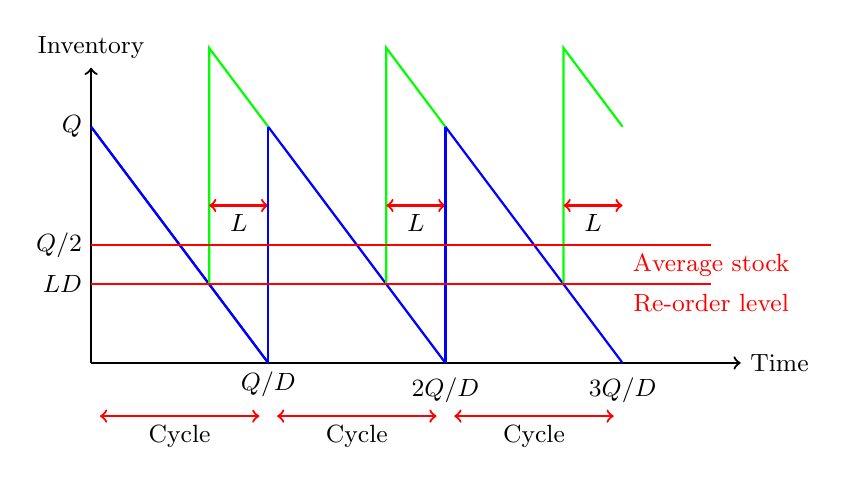
\begin{tikzpicture}[x=0.75cm,y=0.015cm]
\small
\draw[thick,->] (0,0) -- (11,0) node[right] {Time};
\draw[thick,->] (0,0) -- (0,250) node[above] {Inventory};
\draw[] (0,200) -- (0,200) node[left] {$Q$};
\draw[color=blue,thick] (0,200) -- (3,0);
\draw[] (3,0) node[below] {$Q / D$};
\foreach \y in {1,...,3}{
	\draw[color=blue,thick] (3*\y-3,200) -- (3*\y,0);
	\draw[color=green,thick] (3*\y-3+2,200/3) -- (3*\y-3+2,200/3*4) -- (3*\y,200);
	\draw[color=red,thick,<->] (3*\y-3+2,200/3*2) -- (3*\y,200/3*2);
	\draw[] (3*\y-3+2.5,200/3*2) node[below] {$L$};}
\foreach \y in {1,2}{
	\draw[color=blue,thick] (3*\y,0) -- (3*\y,200);}
\foreach \y in {2,3}{
	\draw[] (3*\y,-5) node[below] {\y $Q/D$};}
\draw[] (0,100) node[left] {$Q / 2$};
\draw[color=red,thick] (0,100) -- (10.5,100) node[below] {Average stock};
\draw[] (0,200/3) node[left] {$L D$};
\draw[color=red,thick] (0,200/3) -- (10.5,200/3) node[below] {Re-order level};
\foreach \y in {0,...,2}{
	\draw[color=red,thick,<->] (3*\y+0.15,-45) -- (3*\y+3-0.15,-45);
	\draw[] (3*\y+1.5,-45) -- (3*\y+1.5,-45) node[below] {Cycle};}
\end{tikzpicture}
\end{center}
    
This new policy can be described in a simple way by introducing the
concept of \emph{inventory position}, that is, all stock on-hand plus
the replenishments under way. The green graph above illustrates the
inventory position $IP$. When $IP$ hits the lead time demand $L D$,
i.e., the lead time $L$ times the demand $D$, we should order
$Q$. During the lead time $L$ the demand will be met from on-hand
stock. When the replenishment arrives a lead time $L$ later, it
arrives just in time to meet the demand again .
  \end{comment}
\end{exercise}

\begin{exercise}

How can we decompose leadtime?

\begin{comment}
TBD
\end{comment}

\end{exercise}



\begin{exercise}
  What would happen if it is allowed to backorder demand, in other
  words $b>0$, but $\pi = 0$? (We set $L=0$ again.)
  \begin{comment}
\begin{center}
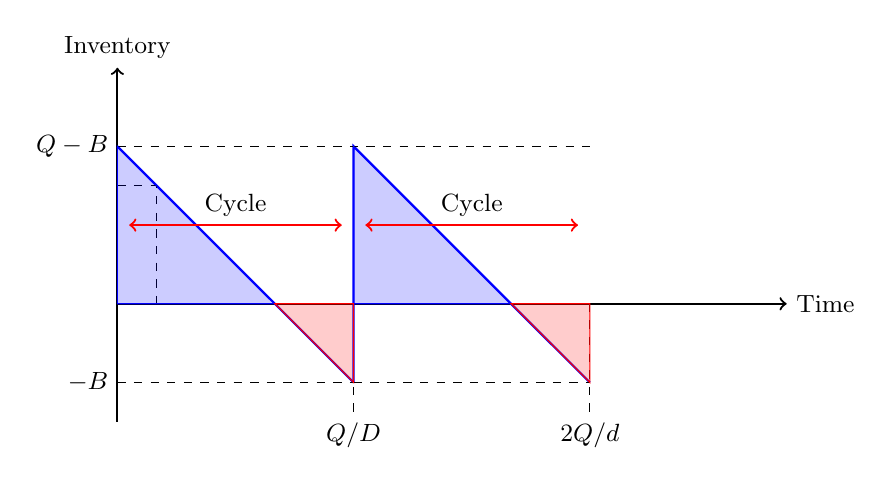
\begin{tikzpicture}[x=1cm,y=0.01cm]
\small

\draw[thick,->] (0,0) -- (8.5,0) node[right] {Time};
\draw[thick,->] (0,-150) -- (0,300) node[above] {Inventory};

\draw[] (0,200) node[left] {$Q - B$};

\draw[color=blue,thick] (0,200) -- (3,-100);

\draw[] (0,-100) node[left] {$-B$};
\draw[dashed] (0,-100) -- (3,-100);

%\draw[] (0,150) node[left] {$Q - B - Dt$};
%\draw[] (0.5,0) node[below] {$t$};
\draw[dashed] (0,150) -- (0.5,150) -- (0.5,0);

%\draw[] (2,0) node[below] {$(Q - B) / d$};

\draw[dashed] (3,0) -- (3,-140) node[below] {$Q / D$};

\draw[color=blue,thick] (3,-100) -- (3,200) -- (6,-100);
%\draw[] (5,0) node[below] {$(2Q - B) / d$};
\draw[dashed] (6,0) -- (6,-140) node[below] {$2Q / d$};
\draw[dashed] (0,200) -- (6,200);
\draw[dashed] (3,-100) -- (6,-100);

\draw [draw=blue,fill=blue,fill opacity=0.2] (0,0) -- (0,200) -- (2,0) -- cycle;
\draw [draw=blue,fill=blue,fill opacity=0.2] (3,0) -- (3,200) -- (5,0) -- cycle;
\draw [draw=red,fill=red,fill opacity=0.2] (2,0) -- (3,-100) -- (3,0) -- cycle;
\draw [draw=red,fill=red,fill opacity=0.2] (5,0) -- (6,-100) -- (6,0) -- cycle;

\foreach \y in {0,1}{
	\draw[color=red,thick,<->] (3*\y+0.15,100) -- (3*\y+3-0.15,100);
	\draw[] (3*\y+1.5,100) node[above] {Cycle};}
\end{tikzpicture}
\end{center}

The blue area is
\begin{equation*}
\frac12  \text{height}\cdot\text{base} = \frac12 (Q-B)\frac{(Q-B)}{D}=\frac{(Q-B)^2}{2D}
\end{equation*}
while the red area is
\begin{equation*}
  \frac12 B \frac{B}{D}=\frac{B^2}{2D}.
\end{equation*}
Thus, the time average cost is the total cost divided by the cycle lenght $Q/D$:
\begin{equation*}
  \begin{split}
  F(Q) 
&= \frac{D}{Q}A + \frac{h(Q-B)^2/2D}{Q/D} + \frac{b B^2/2D}{Q/D} \\
&= \frac{D}{Q}A + h\frac{(Q-B)^2}{2Q} + b \frac{B^2}{2Q}.
  \end{split}
\end{equation*}
Check that by setting $B=0$ you get the old EOQ result.
\end{comment}
\end{exercise}

\begin{exercise}
  What happens to the optimal cost if you allow for backorders?  What
  will happen to the optimal order quantity $Q$, will it become larger or smaller? 
  \begin{comment}
    The cost must become lower, since we remove a constraint. 

    Let's see by how much.  This is not so simple, however, because we
    now have two `controls' (or degrees of freedom): the order
    quantity $Q$ and the backorder level $B$. Even though it is
    possible to find a closed form solution for the optimal values of
    $Q$ and $B$, here we satisfy ourselves with a graphical analysis.
    We are going to make a plot of the total cost as a function of $Q$
    for various values of $B$.

    Here is an example. Take $A=100$, $h=0.2$, $D=20$, $B=10$, $b=1$.

\begin{center}
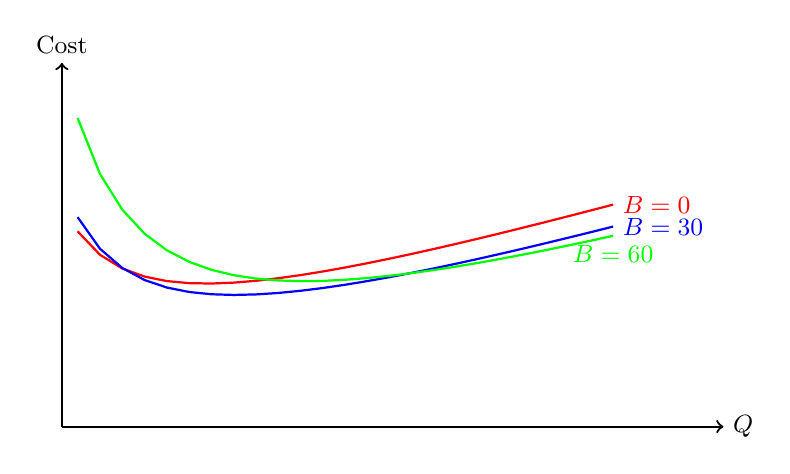
\begin{tikzpicture}[x=0.02cm,y=0.06cm,
declare function = {
f(\Q) = \D*\A/\Q+\h/2*(\Q-\B)/\Q*(\Q-\B)+\b/2*\B/\Q*\B; }
]
\small
\def\A{100} 
\def\h{0.2} 
\def\D{20} 
\def\b{1}
%\def\B{0}
%\pgfmathsetmacro{\f}{sqrt(2)*sqrt(\A)*sqrt(\D)*sqrt(\h)}	
\draw[thick,->] (50,-2) -- (470,-2) node[right] {$Q$};
\draw[thick,->] (50,-2) -- (50,75) node[above] {Cost};
%\draw[color=red,thick,domain=60:400] plot function{\D*\A/x+\h*x/2} node[right] {$B=0$};
%\draw[color=red,thick,domain=60:400] plot (\x,{\D*\A/\x+1*pow(\x,2)}) node[right] {$B=0$};
\def\B{0}
\draw[color=red,thick,domain=60:400] plot (\x,{f(\x)}) node[right] {$B=\B$};
\def\B{30}
\draw[color=blue,thick,domain=60:400] plot (\x,{f(\x)}) node[right] {$B=\B$};
\def\B{60}
\draw[color=green,thick,domain=60:400] plot (\x,{f(\x)}) node[below] {$B=\B$};
% \begin{axis}
% \addplot {f(x)};
% \end{axis}
\end{tikzpicture}
\end{center}


We see that the curve related to $B=30$, i.e., the
blue curve, achieves the lowest point of each of the three graphs.
The minimum of the blue curve is realized a bit to the right of the
minimum of the $B=0$ curve, i.e., the red curve.  Thus, from the
graphs, by setting $B=30$ and $Q$ a bit larger than the optimal value
for the EOQ model, we can lower the cost a bit.

% \begin{tikzpicture}[domain=-1:1,yscale=2,xscale=4,smooth]
% %\fill[gray] (-1.2,-1.2) rectangle (1.2,2.5);
% \draw[very thin] (-1.1,-1.1) grid[step=.5] (1.1,2.4);
% \draw[thick,->] (-1.2,0) -- (1.2,0);
% \draw[thick,->] (0,-1.2) -- (0,2.5);
% \draw[color=red] plot[id=1] function{cos(pi*x)};
% \draw[color=blue,thick] plot[id=2] function{cos(pi*x)+cos(2*pi*x)/2};
% \draw[color=green!50!black,thick] plot[id=3] function{cos(pi*x) + cos(2*pi*x)/2 + cos(3*pi*x)/3};
% \draw[color=yellow,thick] plot[id=4] function{cos(pi*x) + cos(2*pi*x)/2 + cos(3*pi*x)/3 + cos(4*pi*x)/4};
% %\draw<5->[color=cyan,thick] plot[id=5] function{cos(pi*x) + cos(2*pi*x)/2 + cos(3*pi*x)/3 + cos(4*pi*x)/4 + cos(5*pi*x)/5};
% \end{tikzpicture}

% \begin{tikzpicture}[
% declare function={ Nprime(\x)                 = 1/(sqrt(2*pi))*exp(-0.5*(pow(\x,2))); 
%                    d2(\x,\y,\KK,\RR,\SIG)     = (ln(\x/\KK)+(\RR-(pow(\SIG,2)/2)*\y))/(\SIG*(sqrt(\y)));
%                    myfun(\x,\y,\KK,\RR,\SIG)  = exp(-\RR*\y)*Nprime(d2(\x,\y,\KK,\RR,\SIG))/(\x*\SIG*sqrt(\y));
%                  },
% ]
% \begin{axis}[y domain=0.01:0.3,domain=95:105,view={150}{20}]
% \addplot3[surf] {myfun(x,y,100,0,0.09)};
% \end{axis}
% \end{tikzpicture}

  \end{comment}
\end{exercise}

\begin{exercise}
  What would you do if $b=0$, $\pi > 0$ and $h>0$? 
  \begin{comment}

TBD. 
    We have two alternatives. If we decide to keep no inventory, we
    only have to pay for backlogging demand. 

    Demand needs to enter in discrete amounts, for otherwise paying
    $\pi$ per demand becomes a bit strange.
  \end{comment}
\end{exercise}

\begin{exercise}We can also decide to reject demand rather than
  backlog it. Can you sketch the consequences on the behavior of the
  inventory level?  What happens to the order quantity $Q$?  What are
  the consequences in terms of cost, does it become lower or higher?
  \begin{comment}
    The influence on the cost is qualitatively easy. Once again we
    relax a constraint, hence it must be possible to reduce the
    average cost. Again, we are trying to find out by how much. 

    \begin{remark}
      I added this remark as a postscript to the analysis below. The
      solution here is quite messy because, while solving it, I made a
      few mistakes and conceptual errors. Despite this, I decided to
      keep the mistakes in with the aim to show you what went wrong,
      how I saw that things were wrong, and my attempts to repair
      it. The take-away message is that you see that making mistakes
      is part of the learning process\ldots for all of us\ldots
    \end{remark}

    Let's assume we order every $T$ periods.

\begin{center}
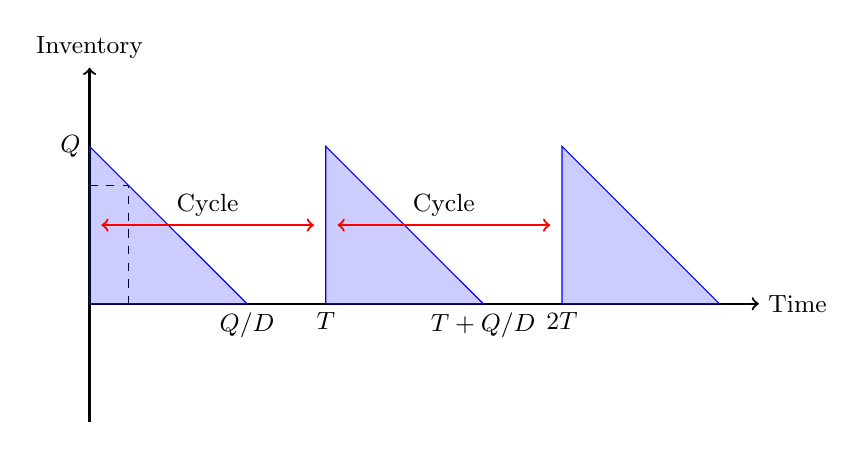
\begin{tikzpicture}[x=1cm,y=0.01cm]
\small

\draw[thick,->] (0,0) -- (8.5,0) node[right] {Time};
\draw[thick,->] (0,-150) -- (0,300) node[above] {Inventory};

\draw[] (0,200) node[left] {$Q$};

%\draw[color=blue,thick] (0,200) -- (3,-100);


%\draw[] (0,150) node[left] {$Q - B - Dt$};
%\draw[] (0.5,0) node[below] {$t$};
\draw[dashed] (0,150) -- (0.5,150) -- (0.5,0);

%\draw[] (2,0) node[below] {$(Q - B) / d$};

\draw[] (2,0) node[below] {$Q/D$};
\draw[] (3,0) node[below] {$T$};

%\draw[color=blue,thick] (3,-100) -- (3,200) -- (6,-100);
%\draw[] (5,0) node[below] {$(2Q - B) / d$};
\draw[] (5,0) node[below] {$T+Q/D$};
\draw[] (6,0) node[below] {$2T$};
%\draw[dashed] (0,200) -- (6,200);
%\draw[dashed] (3,-100) -- (6,-100);

\draw [draw=blue,fill=blue,fill opacity=0.2] (0,0) -- (0,200) -- (2,0) -- cycle;
\draw [draw=blue,fill=blue,fill opacity=0.2] (3,0) -- (3,200) -- (5,0) -- cycle;
\draw [draw=blue,fill=blue,fill opacity=0.2] (6,0) -- (6,200) -- (8,0) -- cycle;

\foreach \y in {0,1}{
	\draw[color=red,thick,<->] (3*\y+0.15,100) -- (3*\y+3-0.15,100);
	\draw[] (3*\y+1.5,100) node[above] {Cycle};}
\end{tikzpicture}
\end{center}

The average cost is the ordering cost plus the inventory cost plus the
cost of lost demand. We already analyzed the cost of the first two
terms. The loss cost is related to all demand lost between the time
$Q/D$ (i.e., the timer it takes the demand to consume $Q$) and the
next order moment $T$. The lost demand is
$DT-Q$. Thus, the average cost becomes
\begin{equation*}
  \begin{split}
  f(Q) 
&= \frac A T + \frac h2 \frac{Q\cdot Q/D}{T}+k \frac{DT-Q}T \\
&= \frac A T + \frac{hQ^2}{2DT}+k (D-\frac QT). 
  \end{split}
\end{equation*}

Take $A=100$, $h=0.2$, $D=20$, $k=1$. As a first attempt, take $T=D/Q^*$ (for the EOQ quantity $Q^*$.) Since $Q^* \approx 141$ and $D=200$, we take $T=200/141\approx 1.4$. \marginpar{This is were I made my first mistake, I copied the wrong numbers.}

\begin{center}
\begin{tikzpicture}[x=0.02cm,y=0.06cm,
declare function = {
f(\Q) = \A/\T+\h/2*\Q/\D*\Q/\T+\k*(\D*\T-\Q); }
]
\small
\def\A{100} 
\def\h{0.2} 
\def\D{20} 
\def\k{1}
%\pgfmathsetmacro{\f}{sqrt(2)*sqrt(\A)*sqrt(\D)*sqrt(\h)}	
\draw[thick,->] (50,-2) -- (470,-2) node[right] {$Q$};
\draw[thick,->] (50,-2) -- (50,75) node[above] {Cost};
\def\T{1.2}
\draw[color=blue,thick,domain=60:400] plot (\x,{f(\x)}) node[right] {$T=\T$};
\def\T{1.5}
\draw[color=red,thick,domain=60:400] plot (\x,{f(\x)}) node[right] {$T=\T$};
\def\T{2.0}
\draw[color=red,thick,domain=60:400] plot (\x,{f(\x)}) node[right] {$T=\T$};
\end{tikzpicture}
\end{center}

Now I wonder why the graph for $T=2$ becomes negative. I guess I did
something wrong, but what?  First I'm checked the cost function. The
only component that can give negative values is
$k(DT-Q)$. \marginpar{As it turned out, I also copied the formula
  incorrectly.} So, when the cost is negative,
I must be considering a combination of $Q$, $D$ and $T$ such that this
term is negative. This only happens when $Q>DT$. But this is strange,
because when $Q>DT$, I am ordering more than the demand that occurs
between two ordering moments, i.e., during the time interval of length
$T$. Clearly then, we must require that $T>Q/D$, which makes
sense. Rechecking also my above estimate for $T$, I notice that I made
stupid algebraic error. It should have been $T=Q^*/D$. For some reason
I also used $D=200$ while it should have been $D=20$. So, let's make a
next attempt with $T=140/20=7$,  use that $Q<DT$, and repair the implementation of the cost function it self (You can't see this in this document, but it is in the source.)

\begin{center}
\begin{tikzpicture}[x=0.02cm,y=0.06cm,
declare function = {
f(\Q) = \A/\T+\h/2*\Q/\D*\Q/\T+\k*(\D-\Q/\T); }
]
\small
\def\A{100} 
\def\h{0.2} 
\def\D{20} 
\def\k{1}
%\pgfmathsetmacro{\f}{sqrt(2)*sqrt(\A)*sqrt(\D)*sqrt(\h)}	
\draw[thick,->] (50,-2) -- (470,-2) node[right] {$Q$};
\draw[thick,->] (50,-2) -- (50,75) node[above] {Cost};
\def\T{7}
\draw[color=blue,thick,domain=60:\D*\T] plot (\x,{f(\x)}) node[right] {$T=\T$};
\def\T{8}
\draw[color=red,thick,domain=60:\D*\T] plot (\x,{f(\x)}) node[right] {$T=\T$};
\def\T{6}
\draw[color=red,thick,domain=60:\D*\T] plot (\x,{f(\x)}) node[right] {$T=\T$};
\end{tikzpicture}
\end{center}

This is too bad: my plotting tool (TikZ) is failing on me, the scales
of the axes are not ok, and I can't read what function belongs to what
graph. In fact, I am now entirely fed up with TikZ, and move to
gnuplot (the tried and tested powertool when it comes to making
plots. With gnuplot I managed to solve the problems in ten minutes. )

\begin{center}
  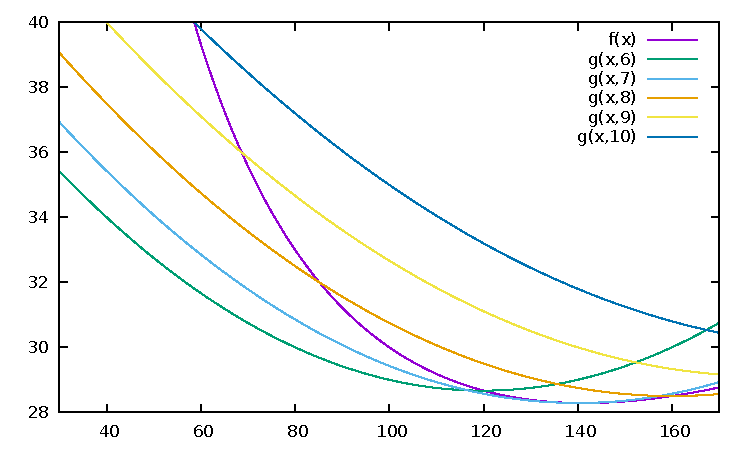
\includegraphics{figures/eoq_loss_0_2}
\end{center}

The situation with $k=0.2$. The $f$ is the graph of the EOQ model, the
$g(x,6)$ is the graph of the cost of the model with loss and with
$T=6$, the $x$ corresponds to the order size $Q$; likewise $g(x,7)$ is
the cost for $T=7$ and so on. We now clearly see that none of the
models with loss achieves a lower cost than the EOQ model with optimal order quantity. 

\begin{center}
  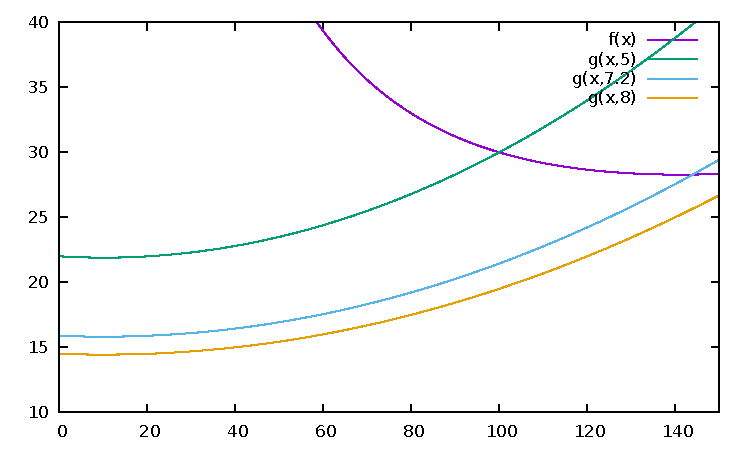
\includegraphics{figures/eoq_loss_0_1}
\end{center}

The situation with $k=0.1$. We now see that when rejecting demand is
pretty cheap, it is best not to order anything: when $Q=0$ the cost is
minimal, hence rejecting all demand seems to be optimal. This is
definitely unexpected!

So, why is that? From the above there seem to be two alternatives,
either order the EOQ and don't reject any demand, or order nothing and
reject all demand.  So, let's trace back the entire analysis.  Indeed,
if we decide to order items and keep them in inventory to satify
demand, then the cost of this must be smaller than the cost of losing
demand. For otherwise, we would simply not be in this business
anyway. So, all in all, this is entirely logical (in hindsight): If
orders are so profitable that you are prepared to keep inventories, it
simply can't be optimal to lose demand. If, however, keeping
inventories is too expensive, it must be optimal not to participate at
all.

Note that this argument is only valid for the case in which everything
is deterministic. In case of stochastic demand, we'll see that
everything changes.

% If we
% reject all demand, then the average cost rate must be $k D$. If, on
% the other hand, we don't want to reject all demand, we order an amount
% $Q$. The cost of ordering is:
% \begin{equation*}
%   \frac A T + \frac{hQ^2}{2DT} - \frac{k Q}{T}.
% \end{equation*}
% Therefore, when this is negative, the overall cost must
% decrease. Thus, if
% \begin{equation*}
%   \frac A T + \frac{hQ^2}{2DT}  < \frac{k Q}{T},
% \end{equation*}
% we must be better off by ordering some amount $Q$. Now it appears that
% all components in this equation are divided by $T$. Removing this
% leads to
% \begin{equation*}
%   A + \frac{hQ^2}{2D}  < k Q.
% \end{equation*}
% But now we see that the cost benefit of ordering $Q$ is independent of
% $T$!



  \end{comment}
\end{exercise}


\begin{exercise}
  Continuing on the above exercise, it might be that items or ordering
  costs are so high that it is better not to `enter the business' at
  all. Can you find a condition to decide whether to keep inventories
  and satisfy demand or reject all demand and have no inventories?
  \begin{comment}
    The cost rate of dropping all demand is $kD$. The cost rate of keeping inventories is, under the EOQ model,  and using that the optimal order quantity $Q^* = \sqrt{2AD/h}$, 
    \begin{equation*}
      \begin{split}
      f(Q^*)
 &= A \frac{D}{Q^*} + \frac h 2 Q \\
 &= A \frac{D}{\sqrt{2AD/h}} + \frac h 2 \sqrt{\frac{2AD}h} \\
 &= A D \sqrt{\frac{h} {2AD}} + \frac h 2 \sqrt{\frac{2AD}h} \\
 &=  \sqrt{\frac {AhD}{2}} + \sqrt\frac{ADh}2 \\
 &=  2\sqrt{\frac {AhD}{2}} \\
 &=  \sqrt{2AhD}.
      \end{split}
    \end{equation*}
When the cost rate of rejecting demand is lower than the cost rate of keeping inventories, we reject the demand, that is, when
\begin{equation*}
kD < \sqrt{2AhD}.
\end{equation*}
We can simplity this a bit to $k^2D^2 < 2AhD$, from which we get
\begin{equation*}
  k^2 D < 2 A h.
\end{equation*}
Thus, when the demand is really small, or the reject cost $k$ is
small, we reject demand. 
  \end{comment}
\end{exercise}


\begin{exercise}
  What if we have quantity discounts? What would you do?  
  \begin{comment}
We would need to analyze various alternatives, one alternative for each `ordering regime', since now the ordering cost depends on  the amount we are going to order.

\paragraph{All-unit discounts}

\begin{center}
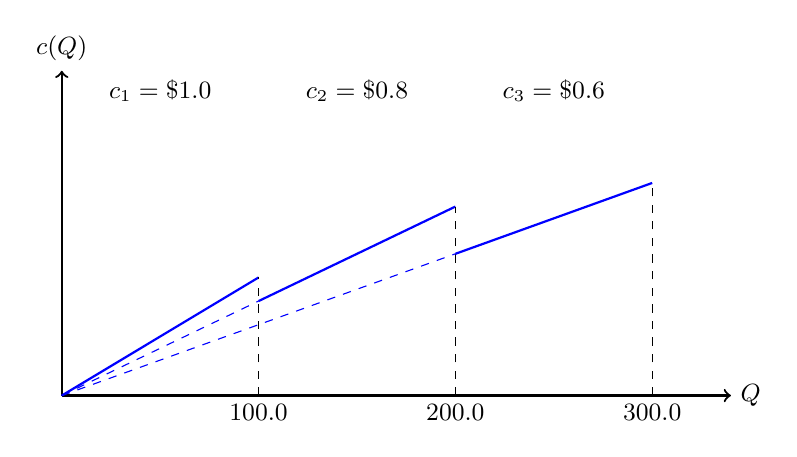
\begin{tikzpicture}[x=0.025cm,y=0.015cm]
\small
\draw[thick,->] (0,0) -- (340,0) node[right] {$Q$};
\draw[thick,->] (0,0) -- (0,275) node[above] {$c(Q)$};
\def\w{100}
\foreach \n/\a in {1/1.0,2/0.8,3/0.6}{
	\pgfmathsetmacro{\s}{(\n-1)*\w}	
	\pgfmathsetmacro{\e}{\n*\w}
	\draw[thick,color=blue,domain=\s:\e] plot (\x,{\a*\x});
	\draw[dashed,color=blue,domain=0:{\s+0.01}] plot (\x,{\a*\x});
	\draw[] (\e,0) -- (\e,0) node[below] {$\e$};
	\draw[dashed] (\e,0) -- (\e,\e*\a);
	\draw[] ({(\s+\e)/2},275) -- ({(\s+\e)/2},275) node[below] {$c_{\n} = \mathdollar\a$};}
\end{tikzpicture}
\end{center}

Average cost per unit time:
\begin{align*}
f(Q) 
& = Kd / Q + cd + hQ/2 \\
& = Kd / Q + cd + \alpha cQ / 2 \quad (h = \alpha c)
\end{align*}

Average cost per unit time:
\begin{equation*}
f(Q) = 
\begin{cases}
Kd / Q + c_1 d + \alpha c_1 Q / 2 & \text{if } 0 \leq Q < Q_1 \\
Kd / Q + c_2 d + \alpha c_2 Q / 2 & \text{if } Q_1 \leq Q < Q_2 \\
Kd / Q + c_3 d + \alpha c_3 Q / 2 & \text{if } Q_2 \leq Q 
\end{cases}
\end{equation*}

\begin{equation*}
f(Q) = 
\begin{cases}
Kd / Q + 1.0 d + \alpha 1.0 Q / 2 & \text{if } 0 \leq Q < 100 \\
Kd / Q + 0.8 d + \alpha 0.8 Q / 2 & \text{if } 100 \leq Q < 200 \\
Kd / Q + 0.6 d + \alpha 0.6 Q / 2 & \text{if } 200 \leq Q 
\end{cases}
\end{equation*}

\begin{equation*}
f(Q) = 
\begin{cases}
2000 / Q + 20 + 0.10 Q & \text{if } 0 \leq Q < 100 \\
2000 / Q + 16 + 0.08 Q & \text{if } 100 \leq Q < 200 \\
2000 / Q + 12 + 0.06 Q & \text{if } 200 \leq Q 
\end{cases}
\end{equation*}

\begin{itemize}
\item $c_1 = \mathdollar 1.0$, $c_2 = \mathdollar 0.8$, $c_3 = \mathdollar 0.6$
\item $Q_1 = 100$, $Q_2 = 200$
\end{itemize}

\begin{itemize}
\item $K = \mathdollar 100$
\item $\alpha = 0.2$, $d = 20$ units
\end{itemize}

\begin{center}
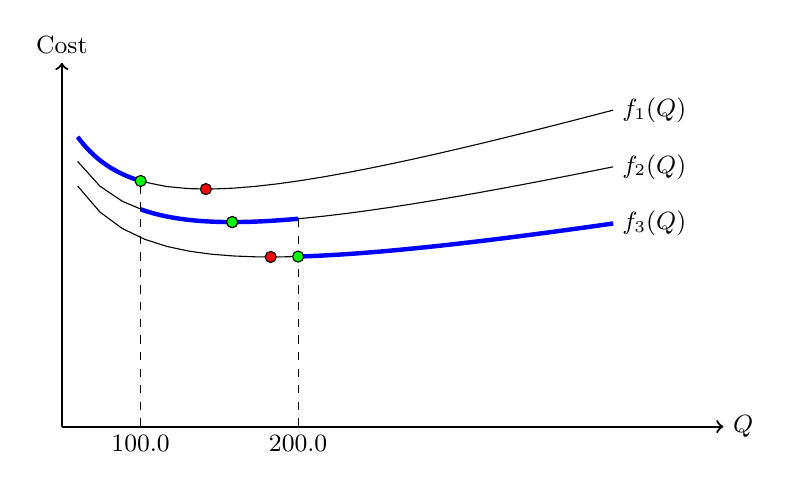
\begin{tikzpicture}[x=0.02cm,y=0.06cm]
\small
\def\c{1} 
\def\K{100} 
\def\h{0.2} 
\def\d{20} 
\def\alpha{0.2}
\def\w{100}
\draw[thick,->] (50,-2) -- (470,-2) node[right] {$Q$};
\draw[thick,->] (50,-2) -- (50,75) node[above] {Cost};
\foreach \n/\c in {1/1.0,2/0.8,3/0.6} {
	\pgfmathsetmacro{\h}{\alpha*\c}	
	\pgfmathsetmacro{\Q}{sqrt(2)*sqrt(\K)*sqrt(\d)/sqrt(\h)}
	\pgfmathsetmacro{\f}{sqrt(2)*sqrt(\K)*sqrt(\d)*sqrt(\h)+\c*\d}	
	\pgfmathsetmacro{\s}{(\n-1)*\w}	
	\pgfmathsetmacro{\e}{\n*\w}

	\draw[domain=60:400] plot (\x,{\d*\K/\x+\c*\d+\h*\x/2}) node[right] {$f_{\n}(Q)$};

	\ifnum\n<3
		\draw[color=blue,ultra thick,domain={max(60,\s}:\e] plot (\x,{\d*\K/\x+\c*\d+\h*\x/2});
		\draw[dashed] (\e,-2) -- (\e,{\d*\K/\e+\c*\d+\h*\e/2});
		\draw (\e,-2) node[below] {$\e$};
	\else
		\draw[color=blue,ultra thick,domain={max(60,\s}:400] plot (\x,{\d*\K/\x+\c*\d+\h*\x/2});
	\fi

	\draw [fill=red] (\Q,\f) circle (2pt);

	\pgfmathparse{int(\Q-\s)}
	\ifnum \pgfmathresult < 0
		\draw [fill=green] (\s,{\d*\K/\s+\c*\d+\h*\s/2}) circle (2pt);
	\fi
	\pgfmathparse{int(\Q-\e)}
	\ifnum \pgfmathresult > 0
		\draw [fill=green] (\e,{\d*\K/\e+\c*\d+\h*\e/2}) circle (2pt);
	\fi
	\pgfmathparse{int((\Q-\e)*(\Q-\s))}
	\ifnum \pgfmathresult < 0
		\draw [fill=green] (\Q,\f) circle (2pt);
	\fi
}
\end{tikzpicture}
\end{center}

Optimization:
\begin{itemize}
\item global optimum $\rightarrow$ check breakpoints and local minimums and compare average total costs
\end{itemize}


\paragraph{incremental discounts}

\begin{center}
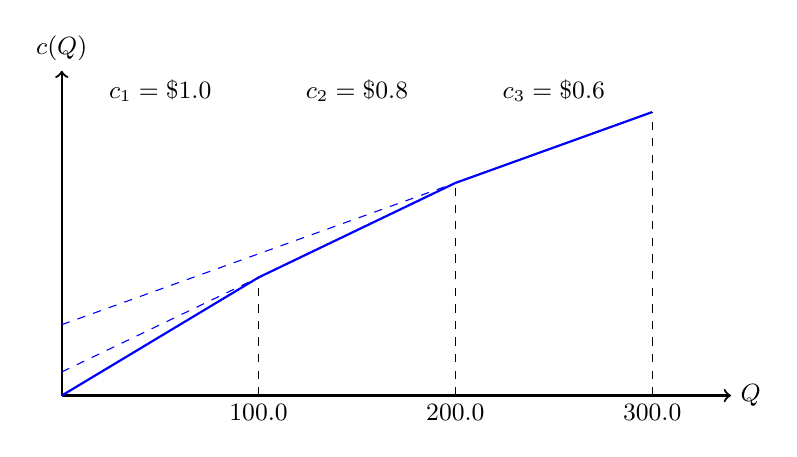
\begin{tikzpicture}[x=0.025cm,y=0.015cm]
\small
\draw[thick,->] (0,0) -- (340,0) node[right] {$Q$};
\draw[thick,->] (0,0) -- (0,275) node[above] {$c(Q)$};
\def\w{100}
\pgfmathsetmacro{\b}{0}
\foreach \n/\a/\b in {1/1.0/0,2/0.8/20,3/0.6/60}{
	\pgfmathsetmacro{\s}{(\n-1)*\w}	
	\pgfmathsetmacro{\e}{\n*\w}
	\draw[thick,color=blue,domain=\s:\e] plot (\x,{\a*\x+\b});
	\draw[dashed,color=blue,domain=0:{\s+0.01}] plot (\x,{\a*\x+\b});
	\draw[] (\e,0) -- (\e,0) node[below] {$\e$};
	\draw[dashed] (\e,0) -- (\e,\e*\a+\b);
	\draw[] ({(\s+\e)/2},275) -- ({(\s+\e)/2},275) node[below] {$c_{\n} = \mathdollar\a$};}
\end{tikzpicture}
\end{center}

Average cost per unit time:
\begin{align*}
f(Q) 
& = Kd / Q + cd + hQ / 2 \\
& = Kd / Q + c(Q)d/Q + \alpha c(Q)/2 \quad (c = c(Q)/Q, h = \alpha c)
\end{align*}

Average variable cost:

\begin{equation*}
c(Q) = 
\begin{cases}
c_1 Q & \text{if } 0 \leq Q < Q_1 \\
c_1 Q_1 + c_2(Q - Q_1) & \text{if } Q_1 \leq Q < Q_2 \\
c_1 Q_1 + c_2(Q_2 - Q_1) + c_3(Q - Q_2) & \text{if } Q_2 \leq Q 
\end{cases}
\end{equation*}


\begin{equation*}
c(Q) = 
\begin{cases}
Q & \text{if } 0 \leq Q < 100 \\
20 + 0.8Q & \text{if } 100 \leq Q < 200 \\
60 + 0.6Q & \text{if } 200 \leq Q 
\end{cases}
\end{equation*}

Average cost per unit time:

\begin{equation*}
f(Q) = Kd / Q + c(Q)d / Q + \alpha c(Q) / 2
\end{equation*}

\begin{equation*}
f(Q) = 2000 / Q + c(Q)20 / Q + 0.1 c(Q)
\end{equation*}

\begin{itemize}
\item $c_1 = \mathdollar 1.0$, $c_2 = \mathdollar 0.8$, $c_3 = \mathdollar 0.6$
\item $Q_1 = 100$, $Q_2 = 200$
\end{itemize}

\begin{itemize}
\item $K = \mathdollar 100$
\item $\alpha = 0.2$, $d = 20$ units
\end{itemize}

Average cost per unit time: (convex for each segment)
\begin{equation*}
f(Q) = 
\begin{cases}
2000 / Q + 20 + 0.10Q & \text{if } 0 \leq Q < Q_1 \\
2400 / Q + 18 + 0.08Q & \text{if } Q_1 \leq Q < Q_2 \\
3200 / Q + 18 + 0.06Q & \text{if } Q_2 \leq Q 
\end{cases}
\end{equation*}

\begin{center}
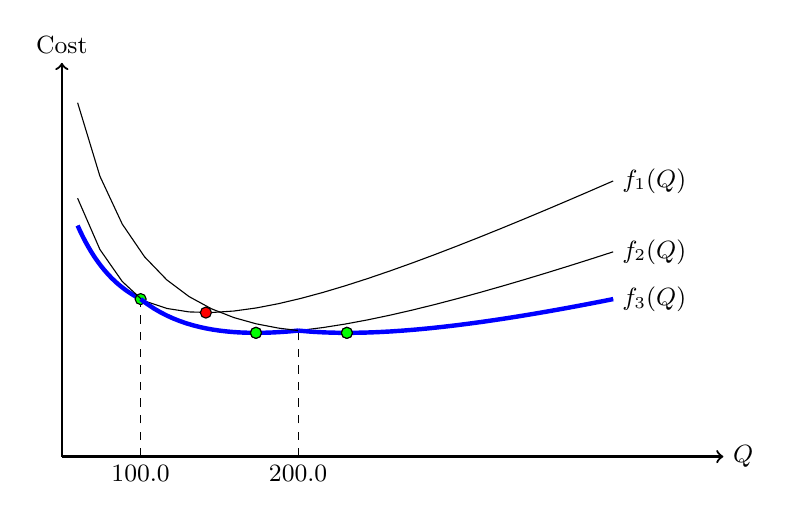
\begin{tikzpicture}[x=0.02cm,y=0.10cm]
\small
\def\c{1} 
\def\K{100} 
\def\h{0.2} 
\def\d{20} 
\def\alpha{0.2}
\def\w{100}
\draw[thick,->] (50,30) -- (470,30) node[right] {$Q$};
\draw[thick,->] (50,30) -- (50,80) node[above] {Cost};
\foreach \n/\a/\b/\c in {1/2000/20/0.1,2/2400/18/0.08,3/3200/18/0.06} {
	\pgfmathsetmacro{\Q}{sqrt(\a)/sqrt(\c)}	
	\pgfmathsetmacro{\f}{\a/\Q+\b+\c*\Q}	
	\pgfmathsetmacro{\s}{(\n-1)*\w}	
	\pgfmathsetmacro{\e}{\n*\w}

	\draw[domain=60:400] plot (\x,{\a/\x+\b+\c*\x}) node[right] {$f_{\n}(Q)$};

	\ifnum\n<3
		\draw[color=blue,ultra thick,domain={max(60,\s}:\e] plot (\x,{\a/\x+\b+\c*\x});
		\draw[dashed] (\e,30) -- (\e,{\a/\e+\b+\c*\e});
		\draw (\e,30) node[below] {$\e$};
	\else
		\draw[color=blue,ultra thick,domain={max(60,\s}:400] plot (\x,{\a/\x+\b+\c*\x});
	\fi

	\draw [fill=red] (\Q,\f) circle (2pt);

	\pgfmathparse{int(\Q-\s)}
	\ifnum \pgfmathresult < 0
		\draw [fill=green] (\s,{\a/\s+\b+\c*\s}) circle (2pt);
	\fi
	\pgfmathparse{int(\Q-\e)}
	\ifnum \pgfmathresult > 0
		\draw [fill=green] (\e,{\a/\e+\b+\c*\e}) circle (2pt);
	\fi
	\pgfmathparse{int((\Q-\e)*(\Q-\s))}
	\ifnum \pgfmathresult < 0
		\draw [fill=green] (\Q,\f) circle (2pt);
	\fi
}
\end{tikzpicture}
\end{center}

Optimization:
\begin{itemize}
\item global optimum $\rightarrow$ check breakpoints and local minimums and compare average total costs
\end{itemize}
  \end{comment}
\end{exercise}



\begin{exercise}
EOQ with joint ordering
  \begin{comment}
    TBD
  \end{comment}
\end{exercise}

\begin{exercise}
  Consider the setting of the EOQ model but now with batchsize
  constraints, that is, the order quantity is in multiples of some number $q$, say. Can you make a formula for the cost, and find the minimum?
  \begin{comment}
This is, in fact, really easy. Suppose we order $n$ times the minimal order quantity $q$. Then, for a yearly demand $D$, ordering cost $A$, and inventory cost $h$, we pay per year
\begin{equation*}
  A \frac{D}{nq} + h\frac{nq}2 = A\frac{D/q}n + hq\frac{n}2.
\end{equation*}
But this is precisely the normal EOQ model with demand $D'=D/q$ and inventory cost $h'=hq$. Thus, the optimal number of batches to order is:
\begin{equation*}
  n^2 = \frac{2D'A}{h'} = \frac{2AD/q}{hq} = \frac{2AD}{hq^2}.
\end{equation*}
Hence, the optimal $n$ expressed in the EOQ quantity $Q^*$ is 
\begin{equation*}
  n = \sqrt{\frac{2AD}{h}}\frac1q=\frac{Q^*}q.
\end{equation*}
  \end{comment}
\end{exercise}


\begin{exercise}
EOQ with yield loss
  \begin{comment}
    TBD
  \end{comment}
\end{exercise}

\begin{exercise}
EOQ with lower salvage value
  \begin{comment}
    TBD
  \end{comment}
\end{exercise}


\begin{exercise}
EOQ with constraints on cycle length

EOQ under periodic review rather than continuous review.

Constraints on when to order, order moment.

  \begin{comment}
    TBD
  \end{comment}
\end{exercise}


\begin{exercise}
  EOQ with positive replenishment lead time and variance in the lead
  time.

  \begin{comment}
    TBD

Suddenly we have to deal with safety stock!
  \end{comment}
\end{exercise}

\begin{exercise}
  Suppose that the delivery rate of the items we order is not
  `infinite', as it is in the EOQ setting (recall, in the EOQ we
  assume instantaneous deliveries). If we have a machine that
  replenishes the FGI we have to take into account the production
  rate, $r$ say. If it costs $K$ to switch on the machine, when do you switch the machine on or off?
  \begin{comment}
    An easy policy is to switch the machine on when the FGI level hits
    some level $Q$, and switch it off when the level is $0$. Of course
    we need to assume that $D<r$, i.e., the production rate is larger
    than the demand rate $D$. 

    To find an expression to cover this situation we can reason like
    this.  When the machine is on, inventory increases at rate
    $r-D$. If we keep it on for $T$ time units, then the inventory
    level is $T(r-D)$ when we switch off. The time until the inventory
    hits 0 is then $T(r-D)/D$, since we start with an inventory level
    $T(r-D)$ after switching off and the demand rate is $D$. Thus, the total cycle length is
    \begin{equation*}
      T + \frac{T(r-D)}D = T + T(\frac{r}D-1) = T + T\frac r D - T = T\frac r D.
    \end{equation*}

    What is, in the EOQ, the average inventory cost? It is half the
    maximal height times $h$, i.e., $hQ/2$. In our present case, the
    maximal height is $T(r-D)$. Thus the average inventory cost must
    be  $hT(r-D)/2$. 

    The ordering cost in the EOQ is $A$ times the order frequency, i.e., $A D/Q$. Here the time between two `order' moments (switching moments) is $Tr/D$. Hence, the frequency is $D/rT$ and the average switching cost is $K D/rT$. 

All in all we get for the average cost
\begin{equation*}
  \frac{h(r-D)}2 T + \frac{K}r \frac DT.
\end{equation*}
This is similar to the EOQ model with $h'=h(r-D)$ and $A=K/r$. But then the optimal $T$ must be given by
\begin{equation*}
  T = \sqrt{\frac{2AD}{h'}} = \sqrt{\frac{2DK/r}{h(r-D)}}=\sqrt{\frac{2DK}{hr(r-D)}}.
\end{equation*}
  \end{comment}
\end{exercise}


\begin{exercise}
EOQ with variable demand.
  \begin{comment}
    TBD
  \end{comment}
\end{exercise}

\begin{exercise}
Wagner Whitin
  \begin{comment}
    TBD
  \end{comment}
\end{exercise}

\begin{exercise}
Silver meal
  \begin{comment}
    TBD
  \end{comment}
\end{exercise}

\begin{exercise}
Where to put the I/O interface? For what product/item?
  \begin{comment}
    TBD
  \end{comment}
\end{exercise}

\begin{exercise}
  What is the difference between continuous and period review? Why/when to prefer one over the other?
  \begin{comment}
    TBD
  \end{comment}
\end{exercise}

\begin{exercise}
  What is the difference between fixed order and order-up-to policies?
  Why/when to prefer one over the other?
  \begin{comment}
    TBD

Order quantities

  \end{comment}
\end{exercise}

\begin{exercise}
  What  different type of service level can you define?
  Why/when to prefer one over the other?
  \begin{comment}
    TBD

e.g. cycle service level.
  \end{comment}
\end{exercise}

\begin{exercise}
  Why to use safefy stock? What is it? 
  \begin{comment}
    TBD
  \end{comment}
\end{exercise}

\begin{exercise}
  Are lead times typically (approximately) constant ore variable?
  \begin{comment}
    TBD
  \end{comment}
\end{exercise}



\subsection{Strategic impact of short leadtimes/small inventories,
  what if lead time is a control?}

You run a pharmaceutical company. The medicines you sell need to be
packaged. The price quotation of the company that prints the packages
depends on the order size $Q$.
  \begin{itemize}
  \item If $Q$ covers 2 weeks of demand: price per unit is 1.15 Euro
  \item If $Q$ covers 1 month of demand: price per unit is 1. Euro
  \item If $Q$ covers 2 months of demand: price per unit is 0.95 Euro
  \item If $Q$ covers 3 months of demand: price per unit is 0.9 Euro
  \item If $Q$ covers 6 months of demand: price per unit is 0.85 Euro
  \end{itemize}
The problem is to determine how much to order.

\begin{exercise}
  \begin{itemize}
  \item Include your own storage cost, i.e., packages need to be
    stored as your raw materials inventory.  Suppose the
    inventory cost is $20\%$ per unit per year. Can we now compute the
    inventory cost?  Assume that $D = 12000$ units per year.
  \item Include transportation cost.  Assume that $A = 50$ Euro.
  \end{itemize}
\end{exercise}

\begin{exercise}
Every so often government regulations change. As a result, the entire
stock becomes obsolete. What now?
\begin{comment}
  \begin{itemize}
  \item Use data to make assumptions on the probability that the
    remaining stock will be affected by a regulation change.
  \item Assume that a regulation change occurs, on average, every
    month, and time to implement the change is one month.
  \item If  $Q$ is 2 weeks of demand, then?  there is no problem
  \item If $Q$ is 3 months of demand, then? 
  \end{itemize}
Challenge: Can you compute the optimal order quantity in this situation? 

  \begin{minted}{python}
A = 50.
D = 12000
h = 0.2

def C(Q, p): # return average yearly inventory cost
    # p is price per unit, so that
    # p*h is the inventory cost per unit per year
    cost = A*D/Q + h*p*Q/2.
    return cost

def output(Q, p, period):
    print("Yearly inventory costs %s: %3.2f; price of a batch: %3.2f"%(period, C(Q, p), Q*p))

output(D/24, 1.15, "2 weeks")
#Likewise for the other cases.
  \end{minted}

  \begin{minted}{python}
Yearly costs 2 weeks: 1257.50; batch price: 575.00
Yearly costs 1 month: 700.00; batch price: 1000.00
Yearly costs 2 months: 490.00; batch price: 1900.00
Yearly costs 3 months: 470.00; batch price: 2700.00
Yearly costs 6 months: 610.00; batch price: 5100.00
  \end{minted}

What are the consequences?

  \begin{itemize}
    \item For some customers short lead times are very important. So important
      they are willing to pay significantly more per unit.
    \item For some customers small batch sizes are very important. So
      important they are willing to pay significantly more per unit.
    \item Thus,  it is essential for some/many companies to be
      able to offer short and predictable lead times and produce in
      small batches.
    \item Producing in small batches can be achieved with slack capacity and short setup times and low setup costs.
    \item Short and predictable lead times can be achieved with conwip
      and a order prioritization (priority queues)
  \end{itemize}
\end{comment}
\end{exercise}

\subsection{News boy/vendor model}

We use the notation of Factory Physics (FP). Note that the formulas in
FP are in terms of integrals rather than with summations. We find this
unsatisfactory since it is easy to evaluate summations in excel (or an
other programming environment), and carrying out integration is often
much more difficult. For this reason we derive  results of FP in terms
of summations. 


We develop the newsvendor in stages.  Suppose that a shop sells some
perishable item with a life time of one day. It has to decide one day
ahead, or the morning before the shop opens, on the number of items to
order/make/prepare. The costs are
\begin{align*}
  p_b &= 5, \text{i.e., Buying price of one item} \\
  p_s &= 10,  \text{i.e., Selling  price of one item} \\
  p_e &= 3, \text{i.e, Salvage (end) value of one item} \\
  c_o &= \text{i.e., Overage cost, Cost of having  one  item over at the end of the day} \\
  c_s &= \text{i.e., Shortage cost, Cost of being   one  item short during the day} \\
\end{align*}
Cost for overage or underage are linear.  Let $X$ (a random variable)
be the number of units sold during a particular period, and let $Q$
denote the number of units ordered.  I assume that
$g_i = \P\{ X = i\}$ is given.


\begin{exercise}
  Can you express $c_o$ and $c_s$ in terms of the other cost parameters?
  \begin{comment}
    $c_o = p_b-p_e$ and $c_s = p_s-p_b$. 
  \end{comment}
\end{exercise}


\begin{exercise}
Suppose the daily demand is $X\in \{0,1\}$ and $g(0) = \P(X=0)=1/2 = g(1)$. What would be the best number of items $Q$ to make? 
\begin{comment}
  The profit of the choice $Q=0$ is 0. Now consider $Q=1$. What is the profit?  We pay for one unit, and sell it perhaps. If we don't sell it, we get the salvage value, if we sell it, we get the sales price. Thus, the profit is
  \begin{equation*}
    -p_b 1 + p_s\cdot 1/2 + p_e\cdot 1/2. 
  \end{equation*}
\end{comment}
\end{exercise}

\begin{exercise}
Suppose the daily demand is $X\in \{0,1\}$ and $g(0) = \P(X=0)=1/3 = 1- g(1)$. What would be the best number of items $Q$ to make? 
\begin{comment}
If $Q=1$ we make as a profit:
  \begin{equation*}
    -p_b 1 + p_s\cdot 2/3 + p_e\cdot 1/3 = -5 + 20/3 + 1> 0
  \end{equation*}
So, ordering $Q$ leads to a higher profit than ordering $Q=0$.
\end{comment}
\end{exercise}


\begin{exercise}
  What are the general terms that make up the profit function $Z(Q)$ if you were to order $Q$? 
  \begin{comment}
If you would order an amount $Q$, the profit consist of three terms: 
  \begin{itemize}
  \item expected number sold
  \item expected number left over
  \item order size
  \end{itemize}
  For the expected number of items sold, if the demand $X$ on a day
  turns out to be smaller than $Q$, we sell $X$; if $X>Q$ we only sell
  $Q$. Therefore, the expected sales is
  \begin{equation*}
    \E(\min\{Q,X\}). 
  \end{equation*}
The expected number of items over is $Q$ minus the expected sales: 
  \begin{equation*}
    Q-\E(\min\{Q,X\}) = 
    \E(Q-\min\{Q,X\})
  \end{equation*}
  where the second equation follows from the observation that the
  expected value of a constant is the constant itself, i.e.,
  $Q=\E(Q)$.  Thus, the total profit of buying $Q$ items must be
\begin{equation*}
Z(Q)=  -p_bQ+p_s\E(\min\{Q,X\}) + p_e\E(Q-\min\{Q,X\}).
\end{equation*}
  \end{comment}
\end{exercise}

\begin{exercise}
  Write $\E(X)$, i.e., the expected demand in terms of a summation.
  \begin{comment}
Recall that $\E(X)$ is just a short-hand for
    \begin{equation*}
      \E(X) = \sum_{i=0}^\infty i g(i).
    \end{equation*}
  \end{comment}
\end{exercise}

\begin{exercise}
  Can you write $\E(\min\{X,Q\}$ in terms of probabilities $g(i) = \P(X=i)$?
  \begin{comment}
From the previous exercise,
\begin{equation*}
  \E(\min\{(X,Q\})) = \sum_{i=0}^\infty \min(i,Q)g(i) = \sum_{i=0}^Q i g(i) + \sum_{i=Q+1}^\infty Q g(i).
\end{equation*}
Observe that $\sum_{i=Q+1}^\infty g(i)=\P(X\geq Q+1)$, thus we can simplify the above to
\begin{equation*}
  \E(\min\{(X,Q\})) = \sum_{i=0}^Q i g(i) + Q\P(X\geq Q+1).
\end{equation*}
  \end{comment}
\end{exercise}

\begin{exercise}
  Suppose for our example that the daily demand is $X\in \{0,1,2\}$
  and $g(0) = \P(X=0)=1/4$, $g(1)=1/3$, $g(2)=5/12$. What would be the
  best number of items $Q$ to make?
\begin{comment}
  Now we need to consider three different $Q$'s, $Q=0, 1,$ or $2$.
  Suppose that $Q=1$, then
\begin{equation*}
    \E(\min\{Q,X\}). =   \E(\min\{1,X\}). =   0\P(X=0) + 1\P(X=1)+1\P(X=2) = 1\cdot 1/3+1\cdot 5/12=9/12=3/4.
\end{equation*}
The expected number of items over is $Q$ minus the expected sales: 
  \begin{equation*}
    \E(Q-\min\{Q,X\}) = 1-3/4=1/4
  \end{equation*}
Thus,  for the example, the total profit is
\begin{equation*}
  -5\cdot1 + 10\cdot3/4+3\cdot1/4
\end{equation*}
is the expected profit per day of buying $Q=1$ at the start of the day. 

Once you implement this in excel, it is easy to experiment with
different values of $Q$ and see what is the best choice for $Q$. 
\end{comment}
\end{exercise}


\begin{exercise}
If the demand can be quite big, e.g., $X\in\{0,1,\ldots, 1000\}$, what is the slope of $Z(Q)$ for $Q$ small? What is the slope if $Q$ is big, i.e., near 1000? Assume that the demand distribution is something reasonable.
\begin{comment}
  If $Q=1$ it is very unlikely that the item will not be sold. In fact, we are nearly sure it will be sold, hence, the slope of $Z$ for small $Q$ must be $p_s$. If $Q$ is very large, we are pretty sure the `last item' will not be sold, hence, the slope must be $-p_e$. 
\end{comment}
\end{exercise}

\begin{exercise}
  Suppose there would be a setup cost which you have to pay to order any positive amount $Q>1$. What is then the profit? 
  \begin{comment}
    This is a no-brainer. If the setup cost is $s$, then just subtract
    $s$ from the profit function $Z(Q)$.
  \end{comment}
\end{exercise}

\begin{exercise}
Suppose we would set a certain service level, what is the profit under such a service level? Before we tackle this, what type of service level can we consider? 
\begin{comment}
  Cycle service level $P_1$, i.e., the probability that there are more
  items than demand, i.e., the fraction of periods/days that the shop
  does not run out of stock:
\begin{equation*}
P(X\leq Q) \geq P_1.
\end{equation*}

Another interesting service level is the fraction of demand that is met, i.e., the fill rate must be higher than some level $P_2$:
\begin{equation*}
\E(\min\{Q, X\})/ \E(X) \geq P_2
\end{equation*}
Realize that $\E(\min\{Q, X\})$ is the expected sales, while $\E(X)$ is the expected demand. The average amount of demand met is the sales divided by the demand.
\end{comment}
\end{exercise}

\begin{exercise}
  Now we can consider the profit under setting a certain performance level. How would you compute this?
  \begin{comment}
    If we want to focus on fill rate, first determine $Q$ such that
    $\E(\min\{Q, X\})/ \E(X) \geq P_2$, where $P_2=90\%$ or so. Call
    this $Q_2$. Then compute $Z(Q_2)$ to get the profit. 

    If we want to focus on cycle service level rate, first determine
    $Q$ such that $\P(X\leq Q) \geq P_1$, where $P_1=80\%$ or so. Call
    this quantity $Q_1$. Compute now $Z(Q_1$ to get the profit.
  \end{comment}
\end{exercise}

We next  discuss a few expressions that simplify the implementation of the profit function in excel.

\begin{exercise}
  Explain that $\E( \max\{Q-X, 0\})$ is another expression for the expected number of items over.
  \begin{comment}
    If $Q>X$, we have $Q-X$ over, if $Q\leq X$ we don't have items over. 
  \end{comment}
\end{exercise}

\begin{exercise}
  Write $\E (\max\{Q-X, 0\}) $ as a summation, so that you can implement this in excel.
  \begin{comment}
\begin{equation*}
  \begin{split}
  \E( \max\{Q-X, 0\} )
  &= \sum_{i=0}^\infty \max\{Q-i,0\}\P\{X=i\}\\
  &= \sum_{i=0}^\infty \max\{Q-i,0\}g_i\\
  &= \sum_{i=0}^Q (Q-i) g_i \\
  &= (Q-0) g_0 + (Q-1)g_1+ \cdots (Q-(Q-1))g_{Q-1} + (Q-Q)g_Q\\
  &= (Q-0) g_0 + (Q-1)g_1+ \cdots (Q-(Q-1))g_{Q-1} + 0 g_Q\\
  &= \sum_{i=0}^{Q-1} (Q-i) g_i.
  \end{split}
\end{equation*}
  \end{comment}
\end{exercise}


\begin{exercise}
  Why is $ \E( \max\{X-Q, 0\})$ the expected number of items short?
  \begin{comment}
    If there is a shortage of items, it must be that $X>Q$. The amount short is $X-Q$.
  \end{comment}
\end{exercise}

\begin{exercise}
  Write $\E (\max\{X-Q, 0\}) $ as a summation.
  \begin{comment}
\begin{equation*}
\begin{split}
     \E (\max\{X-Q, 0\} )
   &= \sum_{i=0}^\infty \max\{i-Q,0\}g_i\\
   &= \sum_{i=Q}^\infty (i-Q) g_i \\
   &= \sum_{i=Q+1}^\infty (i-Q) g_i.
\end{split}
\end{equation*}
\end{comment}
\end{exercise}


\begin{exercise}
  Let $Q=3$ and $g_1=g_2\ldots=g_5 = 1/5$. Compute $\theta = \E(X)$, i.e., the expected demand, the expected lost sales and the expected number over.
  \begin{comment}
    \begin{align*}
      \E( X) &= \sum_{i=1}^5 i g_i = 1/5+2/5+\cdots+5/5 = 3, \\
      \E (\max\{X-Q,0\}) &= \sum_{i=Q+1}^5 (i-Q) g_i = (4-3)/5 + (5-3)/5,\\
      \E (\max\{Q-X,0\}) &= \sum_{i=1}^{Q-1} (Q-i) g_i = (3-1)/5 + (3-2)/5.
    \end{align*}
  \end{comment}
\end{exercise}

\begin{exercise}
  Up to now we considered the profit function $Z(Q)$.  Can you
  establish a cost function of the newsvendor problem?
  \begin{comment}
The expected cost resulting from ordering an amount $Q$ follows
from combining the above formulas:
\begin{equation*}
     Y(Q) = c_o  \E( \max\{Q-X, 0\})  +   c_s \E( \max\{X-Q, 0\}) - c_s\E(X).
\end{equation*}
Note that the expected `cost' of selling $\E(X)$ of items should be subtracted from the cost. Since this term does not depend on the decision variable $Q$, it is often left out of the cost function, but formally it should be there.
  \end{comment}
\end{exercise}


\begin{exercise}
  Show that the profit is minus the the cost, i.e., $Z(Q) = -Y(Q)$.
  \begin{comment}
    Here we go:
    \begin{equation*}
      \begin{split}
        Z(Q) 
&=  -p_bQ+p_s\E(\min\{Q,X\}) + p_e\E(Q-\min\{Q,X\}) \\
&=  (p_e - p_b)Q+ p_s(\E(\min\{Q,X\}) - p_e\E(\min\{Q,X\}) \\
&=  (p_e - p_b)Q+ (p_s-p_e)(\E(\min\{Q,X\})\\
&=  -c_oQ+ (c_o+c_s)(\E(\min\{Q,X\})\\
&=  -c_o( Q - \E(\min\{Q,X\})) - c_s(\E(X) - \E(\min\{Q,X\}) + c_s\E(X)\\
&=  -c_o \E(Q-\min\{Q,X\}) - c_s\E(X-\min\{Q,X\}) + c_s\E(X)\\
&=  -c_o \E(\max\{Q-X,0\}) - c_s\E(\max\{X-Q,0\}) + c_s\E(X)\\
&=  -Y(Q).
      \end{split}
    \end{equation*}
Ensure you understand the last two steps. 
  \end{comment}
\end{exercise}

\begin{exercise}
Reproduce the results of the Christmas Lights Example of Factory Physics.
\begin{comment}
  First the data. We also use a library to handle the computations for
  the normal distribution. 


\begin{minted}[mathescape, fontsize=\small, xleftmargin=0.5em]{python}
from scipy.stats import norm
c_o = 5 - 2.5
c_s = 10 - 5
mu = 10000
sigma = 1000
X = norm(loc=mu, scale=sigma) # demand
\end{minted}


The result of the book is easy to produce. 


\begin{minted}[fontsize=\footnotesize, xleftmargin=0.5em, mathescape]{python}
>>> critical_fractile = c_s / (c_o + c_s)
>>>
>>> Q_star = X.ppf(critical_fractile)
>>> Q_star
10430.727299295457

\end{minted}

\end{comment}
\end{exercise}

\begin{exercise}
  In this christmas light example, 
do you think that $\sigma = 1000$ is reasonable? 
  \begin{comment}
    In all honesty, I think it is way too small. I would say that
    $\sigma=5000$ is much more reasonable. The problem is that if you
    would use this larger value, i.e., $\sigma=5000$, in the normal
    distribution, the probability that the demand is
    $\P(X<0)=\Phi((X-\mu)/\sigma < 0$ is not small anymore. However,
    the demand cannot be negative, hence using the normal distribution
    as an approximation of the demand is wrong for such cases. 

    Now this happens quite often: The problems in the books are tuned
    to showcase the simple methods developed in the book. However, as
    soon you have to do something real, the simple tricks all of a
    sudden don't work anymore. 
  \end{comment}
\end{exercise}


\begin{exercise} A Case to  Get rich in one day. 

  \begin{itemize}
  \item You plan to sell Napoleons tomorrow just outside of the
    Duisenberg building.
  \item How much money can you make? 
  \item How many Napoleons would you order today, to sell tomorrow?
  \end{itemize}
  Realize that this case contains a number of the problems related to
  dealing with perishable inventory, e.g., fashion. 

   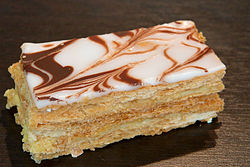
\includegraphics[scale = 1.0]{figures/mille-feuille}

   \begin{comment}
Here are the steps.
  \begin{itemize}
  \item Let's first assume that demand is normally distributed. Then
    we know from FP that $Q$ should be such that
    $G(Q) = c_s/(c_s+c_o)$.
  \item We make some assumptions about the prices. Take $p_s=0.75$,
    $p_b = 0.25$. $p_e=0$. Hence, $c_o = 0.25$, and $c_s = 0.5$.
  \item Thus, the critical fraction is $c_s/(c_s+c_o)=0.5/0.75 = 2/3$.
  \item Now compute $z$ with $\Phi(z)=2/3.$. Hence $z=0.43$.
  \item We also need some idea about the demand. How to get this?
  \item For Napoleons, we don't have yesterday's demand \ldots
  \item Can we use demand data of similar products?  I don't know what
    data to use. I have never tried to sell napoleons.
  \item Can we ask our sales force?  no. We don't have a sales force. 
  \item Last resort: make an educated guess; use powers of ten
    trick. Under this price model, I expect to sell more 1 napoleon,
    also more than 10, 100 might be, 1000 is too much. So, take
    $\mu=100$ as an estimate. Since I am not sure, $\sigma=30$ seems
    reasonable.
  \item If $\mu = 100$ and $\sigma = 30$, then $Q=0.43\sigma + \mu \approx 112$.
  \item Finally, what is the profit $Z(Q)$?
\item With the above formulas you can compute $Z(Q)$,  but let's use handwaving for a quick estimate. 
\item Note that $\min\{Q, X\} \leq X$, hence
  $\E \min\{X, Q\} \leq \E X= \mu$. If $\E \min\{X, Q\}\approx 95$,
  then $Z(112) \approx 95p_s - 100 p_b = 95\cdot 0.75 - 100 \cdot 0.25$.
  Since $95\approx100$, use this to simplify yet more:
  $Z(112) \approx 100(0.75-0.25) = 50$ Euro.
\item There are easier ways to make money!
  \end{itemize}
\end{comment}
\end{exercise}

\begin{exercise}
   Summarize the approach we took to some insight into this napoleon
   case, even though, initially, we had no idea about what profit we
   could make.
   \begin{comment}
Conclusion.
  \begin{itemize}
  \item Determine/estimate relation between demand (distribution) and sales price
  \item Make plots of the profit $Z$ as a function of $Q$, the demand
    distribution, and the sales price.
  \item Choose a $Q$ that makes sense. The existence of an optimal $Q$
    is a \emph{delusion}.
  \item Be aware that salesforce may predict too high demand. They get insentives to sell much, but they are not responsible for overage cost!
  \end{itemize}
   \end{comment}
 \end{exercise}


%%% Local Variables:
%%% mode: latex
%%% TeX-master: "notes_all"
%%% End:

\subsection{Two-Stage Newsvendor Model}

Let us consider a case where we have a two-period planning horizon, rather than one as we had for the newsvendor problem. Here, at the beginning of each period, we  first observe the current inventory level, and then we decide upon the order quantity. Thus, this case  becomes an extension of the newsvendor model, because now we have an extra ordering moment in the middle of the day. 

For convenience, we use the same notation that we used for the single-period newsvendor model. However, we add a period index to the buying and selling prices as well as the demand distribution (i.e. $c_n$, $p_n$, and $g_n(\cdot)$ where $n\in\{1,2\}$), as these can be different in the morning and in the afternoon.

\begin{question}
Suppose the afternoon demand is $D_2\in \{0,1,2\}$ and $g_2(0)=g_2(1)=g_2(2)=1/3$.  Consider  three cases: at the end of the morning you have  0, 1, and 2 items in stock. What would be the best number of items $Q_2$ to order at start of the second period (the afternoon) for each of these cases? (It is perhaps the easiest to use Eq.~\eqref{eq:1}.)

\begin{solution}
	It is obvious that we do not need more than 2 items in the afternoon, because the demand $D_2\leq 2$ always.
	
	\begin{itemize}
	
	\item In the first case (no stock at the end of the morning), our options for $Q_2$ are ordering 0, 1, or 2 items. Take $Q_2=0$ first. Then we see that 
    \begin{equation*}
P(Q_2=0) = (p -c)Q_2  + (s-p)\E{(Q_2-D_2)^+} = (p -c) 0   + (s-p)\E{(0-D_2)^+} = 0.
\end{equation*}
The profit of the choice $Q_2=1$ is 
    \begin{equation*}
P(1) = (p -c)1  + (s-p)\E{(1-D_2)^+}. 
\end{equation*}
Now
\begin{equation*}
  \begin{split}
\E{(1-D_2)^+}
&=(1-0)^+\P{D_2=0} + (1-1)^+\P{D_s=1} + (1-2)^+ \P{D_2=2} \\
&= 1 \P{D_2=0} = 1\cdot 1/3 = 1/3.
  \end{split}
\end{equation*}
Therefore
    \begin{equation*}
P(1) = (p -c)1  + (s-p) 1/3.
  \end{equation*}
Finally, the profit for choice $Q_2=2$ is 
    \begin{equation*}
P(2) = (p -c)2  + (s-p)\E{(2-D_2)^+} = (p-c)2 + (s-p).
\end{equation*}
since
\begin{equation*}
  \begin{split}
\E{(2-D_2)^+}
&=(2-0)^+\P{D_2=0} + (2-1)^+\P{D_s=1} + (2-2)^+ \P{D_2=2} \\
&= 2\cdot 1/3 + \cdot 1/3 = 1.
  \end{split}
\end{equation*}

\item When the inventory at the end of the morning is $1$,  our options are ordering $Q_2=0$ or $Q_2=1$ items. Now if we order $Q_2$, the inventory at the start of the second period is $1+Q_2$. Thefore, the profit function takes the form
    \begin{equation*}
P(Q_2) = (p -c)Q_2  + (s-p)\E{(Q_2+1-D_2)^+}. 
\end{equation*}
Hence, 
    \begin{equation*}
P(0) = (s-p)\E{(1-D_2)^+},
\end{equation*}
and we already computed this expectation above. Also
    \begin{equation*}
P(1) = (p -c)1  + (s-p)\E{(2-D_2)^+}. 
\end{equation*}
  
  \item In the third case, i.e., starting with $2$ items in stock, 
    \begin{equation*}
P(Q_2) = (p -c)Q_2  + (s-p)\E{(Q_2+2-D_2)^+}. 
\end{equation*}
In this case, the  decision is easy as we already have the maximum amount of items that we might possibly need. So the only reasonable choice is $Q_2=0$.  Its profit is 
    \begin{equation*}
P(0) = (s-p)\E{(2-D_2)^+}. 
\end{equation*}
\end{itemize}
\end{solution}
\end{question}

\begin{question}
Explain why the decision on how many items to make in the afternoon depends on the number of items that is left from the morning. 

\begin{solution}
The items that are left from the morning contributes to the profit in the afternoon. That is due to two reasons: (1) We don't have to pay in the afternoon to acquire what we already have in stock as leftovers from the morning (in other words, there is no purchasing cost for leftovers), and (2) if there are more leftovers  than what is actually needed, it is optimal  to not make new items. 
\end{solution}
\end{question}


\begin{question}
Suppose the morning demand is $D_1\in \{0,1,2\}$ and $g_1(0)=g_1(1)=1/4$, $g_1(2)=1/2$; and the afternoon demand is $D_2\in \{0,1\}$ and $g_2(0)=g_2(1)=1/2$. It is not possible to backlog demands, that is,  demands not satisfied in the morning are lost. Also, we have that $c_1=10$, $c_2=12$, $p_1=p_2=20$, and $s=5$. Now, assume that we make 2 items in the morning. What is the expected total profit in the morning and in the afternoon?
\begin{solution}
TBD.

%Let us start with the afternoon. The following are the expected profits (disregarding the purchasing costs) in the afternoon, if the inventory level after making new items is 0, 1, 2, respectively:
%\begin{align*}
%    \text{(start with $0$ item)} \quad  & 0 & = 0 \\
%    \text{(start with $1$ item)} \quad  & p_{s2} \cdot 1/2 + p_e \cdot 1/2 & = 12.5 \\
% 	\text{(start with $2$ items)} \quad  & p_{s2} \cdot 1/2 + p_e \cdot 3/2 & = 17.5
%\end{align*}  
%
%If we make 2 items in the morning, then at the end of the morning 
%\begin{itemize}
%\item with probability $\P(X_1=2)=1/2$ we sell 2 items, make a profit of $-p_{b1} 2 + p_{s1} 2$, and end up with $2-2=0$ items
%\item with probability $\P(X_1=1)=1/4$ we sell 1 item, make a profit of $-p_{b1} 2 + p_{s1} 2$
%
%\end{itemize}
%
%
%
%
%,  we end up with $2-1=1$ items, and with probability $\P(X_1=0)=1/4$ we end up with $2-0=0$ items. 
%
%
%the probability of ending up with 0, 1, 2 items at the end of the morning are: $\P(2-X_1=0)=\P(2-X_1=0)$

\end{solution}

\end{question}

\begin{question}
Let $U(A)$ be a function that returns the expected profit in the afternoon, given that the inventory level after making new items is $A$. What are the general terms that make up this function?
   \begin{solution}
     TBD.
   \end{solution}
\end{question}

\begin{question}
How can one make use of $U(A)$ when deciding the number of items $Q_2$ to make in the afternoon?
   \begin{solution}
     TBD.
   \end{solution}
\end{question}

\begin{question}
Let $V(I)$ be a function that returns the expected profit in the afternoon, given that the inventory level after before making new items is $I$. What are the general terms that make up this function?
   \begin{solution}
     TBD.
   \end{solution}
\end{question}

\begin{question}
Write $U(A)$ and $V(I)$ in terms of probabilities $g_2(i)=\P(X_2=i)$
   \begin{solution}
     TBD.
   \end{solution}
\end{question}

\begin{question}
Let $Z(Q_1)$ be a function that returns the expected profit over the whole day given $Q_1$ items are produced in the morning is $I$. What are the general terms that make up this function?
   \begin{solution}
     TBD.
   \end{solution}
\end{question}

\begin{question}
Write $Z(Q)$ in terms of probabilities $g_1(i)=\P(X_1=i)$
   \begin{solution}
     TBD.
   \end{solution}
\end{question}

\begin{question}
We have so far assumed that the sequence of events over the day were as follows: (1) decide $Q_1$, (2) observe $X_1$, (3) decide $Q_2$, (4) observe $X_2$. How would we set order quantities if the sequence of events were as follows (1) decide $Q_1$ and $Q_2$, (2) observe $X_1$, (3) observe $X_2$.
   \begin{solution}
     TBD.
   \end{solution}
\end{question}

\begin{question}
What is the financial value of having an second ordering moment in the middle of the day, after observing the demand in the morning?
   \begin{solution}
     TBD.
   \end{solution}
\end{question}

\begin{question}
We have thus far considered profit functions $U(A)$, $V(I)$, and $Z(Q_1)$. Can you devise cost functions for the same two-period newsvendor problem?
   \begin{solution}
     TBD.
   \end{solution}
\end{question}

\begin{question}
We have thus far considered profit functions $U(A)$, $V(I)$, and $Z(Q_1)$. Can you devise cost functions for the same two-period newsvendor problem?
   \begin{solution}
     TBD.
   \end{solution}
\end{question}

\begin{question} A Case to  Get rich in \st{one day} two days. 

  \begin{itemize}
  \item You plan to sell Napoleons tomorrow and the next day just outside of the Duisenberg building.
  \item How much money can you make? 
  \item How many Napoleons would you order for each day if you can sell left Napoleons from the first day in the second one?
  \end{itemize}

   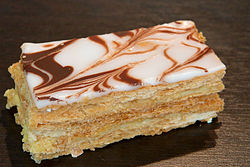
\includegraphics[scale = 1.0]{figures/mille-feuille}
   %\includegraphics[scale = 1.0]{250px-Mille-feuille_20100916}

%   \begin{solution}
%Here are the steps.
%  \begin{itemize}
%  \item Let's first assume that demand is normally distributed. Then
%    we know from FP that $Q$ should be such that
%    $G(Q) = c_s/(c_s+c_o)$.
%  \item We make some assumptions about the prices. Take $p_s=0.75$,
%    $p_b = 0.25$. $p_e=0$. Hence, $c_o = 0.25$, and $c_s = 0.5$.
%  \item Thus, the critical fraction is $c_s/(c_s+c_o)=0.5/0.75 = 2/3$.
%  \item Now compute $z$ with $\Phi(z)=2/3.$. Hence $z=0.43$.
%  \item We also need some idea about the demand. How to get this?
%  \item For Napoleons, we don't have yesterday's demand \ldots
%  \item Can we use demand data of similar products?  I don't know what
%    data to use. I have never tried to sell napoleons.
%  \item Can we ask our sales force?  no. We don't have a sales force. 
%  \item Last resort: make an educated guess; use powers of ten
%    trick. Under this price model, I expect to sell more 1 napoleon,
%    also more than 10, 100 might be, 1000 is too much. So, take
%    $\mu=100$ as an estimate. Since I am not sure, $\sigma=30$ seems
%    reasonable.
%  \item If $\mu = 100$ and $\sigma = 30$, then $Q=0.43\sigma + \mu \approx 112$.
%  \item Finally, what is the profit $Z(Q)$?
%\item With the above formulas you can compute $Z(Q)$,  but let's use handwaving for a quick estimate. 
%\item Note that $\min\{Q, X\} \leq X$, hence
%  $\E \min\{X, Q\} \leq \E X= \mu$. If $\E \min\{X, Q\}\approx 95$,
%  then $Z(112) \approx 95r - 100 c = 95\cdot 0.75 - 100 \cdot 0.25$.
%  Since $95f\approx100$, use this to simplify yet more:
%  $Z(112) \approx 100(0.75-0.25) = 50$ Euro.
%\item There are easier ways to make money!
%  \end{itemize}
%\end{solution}
\end{question}

\begin{question}
Can you generalize the two-period newsvendor case to an arbitrary number of periods?
   \begin{solution}
     TBD.
   \end{solution}
\end{question}

\begin{question}
Can you generalize the two-period newsvendor case to an infinite number of periods?
   \begin{solution}
     TBD.
   \end{solution}
\end{question}


%%% Local Variables:
%%% mode: latex
%%% TeX-master: t
%%% End:





\subsection{Base Stock Model}


\subsubsection{Common notation}
\label{sec:common-notation}

Let $I_t$ denote the on-hand inventory at time $t$, $B_t$ the number
of backorders, $R_t$ the number of out-standing replenishments, and
$X_t := X(t-L,t]$ the demand that occurred during the time interval
$(t-L, t]$. Note that here we write $X_t$ to represent the
random variable $X$ of Factory Physics.
We also write
\begin{equation}
  \label{eq:16}
   G(r) = \P{X_t\leq r},
\end{equation}
and for the average demand during a lead time 
\begin{equation*}
\theta = \E{X_t}.
\end{equation*}

Under the basestock policy the above random variables $I_t, B_t, R_t$
and $X_t$ satisfy a number of important relations.  Recally that
according to the basestock policy we issue a replenishment order as
soon as the re-order level $r$ is hit. First, as for each demand a
replenishment order is sent, it must be that
\begin{equation}
  \label{eq:8}
   R_t = X(t-L, t] = X_t,
\end{equation}
that is, the number of outstanding replenishments at time $t$ equals
all demand $X_t$ that occurred during the previous leadtime.  
Second, as each demand spawns a replenishment, it must be for all time
$t$ that the on-hand inventory $I_t$ plus the number of
replenishments $R_t$ minus all backorders $B_t$ remains
constant. That is, 
\begin{equation*}
I_t + R_t - B_t = \text{ constant}.
\end{equation*}
Third, we do not backorder demand when there is on-hand stock and we
also match backorders (if any) with replenishments as they arrive, it
must hold that
\begin{equation}
  \label{eq:9}
   I_t B_t =0, \text{ for all }  t\geq 0.
\end{equation}
In other words, at any moment in time the on-hand inventory $I_t = 0$ or the
number of backorders $B_t=0$.

Assuming that at time $t=0$,
there are no outstanding replenishments and no backorders, we can
safely assume that $I_0 = r+1$. The above then implies that
\begin{equation}
  \label{eq:7}
   I_t + R_t - B_t = r+1, \text{ for all }  t\geq 0.
\end{equation}


When dealing with positive leadtimes two concepts are very useful. The \emph{inventory level} $\IL_t$ at time $t$ is the basestock level minus the demand: 
\begin{equation}\label{eq:23}
  \IL_t = r+1 - X_t
\end{equation}
Note that from~\eqref{eq:8} and~\eqref{eq:7} it follows that
\begin{equation*}
  \begin{split}
  \IL_t 
&=r - X_t \\
&= (I_t + R_t - B_t) - X_t \\
&= I_t - B_t.
  \end{split}
\end{equation*}


The \emph{inventory position} $\IP_t$ is the inventory level plus all outstanding replenishments:
\begin{equation*}
  \IP_t = \IL_t + R_t.
\end{equation*}
From \eqref{eq:7} we conclude that 
\begin{equation}\label{eq:20}
\IP_t =\IL_t + R_t = I_t - B_t +R_t = r+1.
\end{equation}
Thus, for the basestock mode in continuous time, the inventory position is constant. 


\begin{question}
  What is the reorder level $r$ for a make-to-order inventory system?
\end{question}
\begin{solution}
  In a make-to-order setting, there is no on-hand
  inventory. Production starts when a job comes in. Thus, if we take
  $r=-1$, then when the inventory position hits $-1$, we issue a
  production order. Clearly, $I_t=0$ always, and $B_t$ is the number
  of jobs waiting to get served by production.
\end{solution}


\subsubsection{Computing the Service level}

The service level $S(r)$ is defined as the fraction of demand that
perceives, on arrival, a positive stock level. As we assume that demand
occurs in single units, this fraction is therefore equal to the fraction
of demand served from on-hand stock. We also assume that the arrival
process is given by a Poisson process. Therefore, by the PASTA property,
the fraction of demand served from stock is equal to the (long-run)
fraction of time that the inventory level is positive. Hence,
\begin{equation*}
   S(r) = \P{I_t >0}.
\end{equation*}

Using that $I_t>0$ at time $t$ implies that $B_t = 0$,
it follows from Eq.~\eqref{eq:7} that:
\begin{equation}\label{eq:10}
  \begin{split}
   S(r) &= \P{I_t >0} \\
   &= \P{r+1 + B_t - R_t >0}, \text{  from  \eqref{eq:7}}  \\
   &= \P{r+1 - R_t >0}, \text{ as } B_t = 0, \\
   &= \P{R_t < r+1} \\
   &= \P{R_t \leq r} \\
   & = \P{X_t \leq  r}, \text{from  \eqref{eq:8}}, \\
   &= G(r),  \text{ from \eqref{eq:16}} \\
   &=  \sum_{i=0}^{r} g_i.
  \end{split}
\end{equation}
Thus,
\begin{equation}
  \label{eq:13}
   S(r) = G(r) = \sum_{i=0}^r \P{X_t = i},
\end{equation}
and \emph{not} $G(r+1)$ as in the third edition of Factory Physics.

\subsubsection{Computing the average backorder level}


When does a backorder occur? This happens whenever
\begin{equation}
  \label{eq:11}
  \begin{split}
   \{B_t > 0\} 
&= \{R_t - r-1>0\}, \quad \text{ as } R_t - B_t = r+1\text{ when } B_t >0, \\
&= \{X_t - r-1>0\},\quad \text{ since  } R_t  = X_t.
  \end{split}
\end{equation}
Hence,
\begin{equation*}
   \begin{split}
     B(r) 
   &= \E{B_t} \\
   &= \E{\max\{B_t, 0\}} \\
   &= \E{\max\{R_t - r - 1, 0\}} \\
   &= \E{\max\{X_t - r - 1, 0\}} \\
   &= \sum_{i=r+1}^\infty (i- r -1)\P{X_t = i}\\
   &= \sum_{i=r+1}^\infty (i- r -1)g_i \\
   &= \sum_{i=r+2}^\infty (i- r -1)g_i,
     \end{split}
\end{equation*}
where the last equation follows from the fact that when $i=r+1$,
$i-r-1 =0$. I find the following easier to memorize, hence I use this
in the sequel:
\begin{equation}
  \label{eq:12}
   B(r)  = \sum_{i=r+1}^\infty (i- r -1)g_i.
\end{equation}

Note that in the above formula for $B(r)$ the summation runs to $\infty$, which is a bit problematic for numerical purposes. In the proof below we show that this expression can be rewritten to 
\begin{equation}
  \label{eq:17}
   B(r) 
%= \sum_{i=r+1}^{\infty} \bar G(i)
   = \theta - \sum_{j=0}^{r} \bar G(j)
\end{equation}
where
\begin{equation}
  \label{eq:18}
   \bar G(i) = \P{X>i} = 1 - \P{X\leq i} = 1 - G(i),
\end{equation}
and $\theta = \E{X_t}$. You can skip the proof. 
\begin{proof}
Define first the function
\begin{equation*}
   \1{i< j} =
     \begin{cases}
       1, &\text{  if } i < j, \\
   0, &\text{ else},
     \end{cases}
\end{equation*}
so that we can write
\begin{equation*}
  \sum_{j=0}^\infty \1{j< i-r - 1} = i-r -1.
\end{equation*}
Now, using \eqref{eq:12},
\begin{equation}
  \label{eq:19}
  \begin{split}
       B(r) &= 
   \sum_{i=r+1}^\infty (i-r-1) g(i)   \\
   &= \sum_{i=r+1}^\infty\sum_{j=0}^\infty \1{j < i-r-1}\, g(i)   = 
    \sum_{j=0}^\infty \sum_{i=r+1}^\infty \1{i > j +r + 1}\, g(i)\\
   &= \sum_{j=0}^\infty \sum_{i=j + r+2}^\infty  g(i) = 
   \sum_{j=0}^\infty \P{X_t \geq j + r+2}  \\
   &=\sum_{j=0}^\infty \P{X_t > j + r+1} \\
   &= \sum_{j=0}^\infty \bar G(j+r+1) =\sum_{j=r+1}^\infty  \bar G(j).
  \end{split}
\end{equation}
Finally, this can be simplied a bit by using that
$\sum_{i=0}^\infty \bar G(i) = \theta$:
\begin{equation}
  \label{eq:119}
  \begin{split}
   B(r) 
   &= \sum_{j=r+1}^\infty  \bar G(j) \\
   &= \sum_{j=0}^\infty  \bar G(j) - \sum_{j=0}^{r} \bar G(j)\\
   &= \theta - \sum_{j=0}^{r} \bar G(j)
  \end{split}
\end{equation}
  
\end{proof}
	   

\subsubsection{Computing the expected on-hand inventory}

Taking expectations at the left and right hand side of \eqref{eq:7} we get
\begin{equation*}
  \E{I_t + R_t - B_t} = r+1,
\end{equation*}
from which we find for the on-hand inventory $I_t$: 
\begin{equation}
  \label{eq:6}
  \begin{split}
  \E{I_t}
  &= r+1 - \E{R_t} + \E{B_t}  \\
  & = r + 1 - \E{X_t} + B(r) \\
  & = r + 1 - \theta + B(r) \\
  \end{split}
\end{equation}

Formulas to skip (in edition 3): 2.24, 2.25. 


\subsubsection{Simulation of the basestock inventory model}
\label{sec:simul-basest-invent}

Consider a periodic-time model so that $\IP_t$ is the inventory position at the end of period $t$. Write $D_t = X(t-1, t]$ for the demand that occured in period $t$. (Recall that $X_t = X(t-L, t]$ is the demand during the leadtime $L$, which is not the same as the demand during one period.)
 Then the sequence $\{\IP_i\}$ must satisfy the recursion:
\begin{equation}
  \label{eq:15}
  \IP_t = r+1 = r+1 - D_t + D_t \1{D_t>0}.
\end{equation}
To see this, observe that under the basestock policy the inventory
position is always kept at level $r+1$, c.f., \eqref{eq:20}. Thus, if
the inventory position $\IP_t$ at the end of period $t$ minus the demand
$D_i$ during period $i$ is less than $r+1$, we need to reorder the
shortage. Since the shortage is precisely the demand during period
$t$, i.e., $D_t$, we order $D_t$. (Recall that $\1{D_t>0} = 1$ if
$D_i>0$ and is $0$ otherwise.)

When the leadtime $L$ is one period or more, the replenishments do not arrive right away but $L$ periods later. The consequences of the inventory level are that
\begin{equation}
  \label{eq:21}
  \IL_t = \IL_{t-1} - D_t + D_{t-L}\1{D_{t-L}>0}.
\end{equation}
Thus, what we ordered $L$ periods `ago', we receive `now'.

Once we carry out a simulation for $n$ periods, we can estimate the
performance measure. The average  inventory on-hand is
\begin{equation}
  \label{eq:22}
  I = \frac 1n \sum_{t=1}^n \IL_t\1{\IL_t \geq 0} = \frac1n\sum_{t=1}^n \max{\IL_t, 0}
\end{equation}
the average backlog  is
\begin{equation}
  B = - \frac 1n \sum_{t=1}^n \IL_t\1{\IL_t < 0} = \frac1n\sum_{t=1}^n \max{-\IL_t, 0}
\end{equation}
because $\IL_t<0$ if there are backorders, recall~\eqref{eq:23}. 
The service level is 
\begin{equation}
  \label{eq:22}
  S = \frac 1n \sum_{i=t}^n \1{\IL_t \geq 0},
\end{equation}

\begin{question}\label{q:basestock}
  Suppose the demand during the leadtime is like this:
  \begin{align*}
    \P{X = 0} &= 1/6, & \P{X \leq 0} &= 1/6,  \\
    \P{X = 1} &= 1/5, & \P{X \leq 1} &= 11/30,  \\
    \P{X = 2} &= 1/4, & \P{X \leq 2} &= 37/60, \\
    \P{X = 3} &= 1/8, & \P{X \leq 3} &= 89/120, \\
    \P{X = 4} &= 11/120, & \P{X \leq 4} &= 5/6, \\
    \P{X = 5} &= 1/6, & \P{X \leq 5} &= 1.
  \end{align*}
What is $S(r)$ for $r=0, \ldots, 5$?
\end{question}
\begin{solution}
  \begin{equation*}
    S(r) = G(r) = \sum_{i=0}^r \P{X = i}.
  \end{equation*}
Hence,
\begin{align*}
  r &= 0 \implies S(0) = \P{X \leq 0} = \P{X=0}1/6, \\
  r &= 1 \implies S(1) = \P{X \leq 1} = 1/6 + 1/5 = 11/33, \\
  r &= 2 \implies S(2) = \P{X \leq 2} = 37/60,\\
  r &= 3 \implies S(3) = 89/120, \\
  r &= 4 \implies S(4) = 100/120 = 5/6, \\
  r &= 5 \implies S(5) = 1.
\end{align*}
\end{solution}

\begin{question}\label{q:basestock_theta}
Suppose the demand is a given by the previous exercise. What is $\theta$?
\end{question}
\begin{solution}
  \begin{equation*}
    \theta = \E{X} =
1\cdot 1/5 + \cdots + 5 \cdot 1/6 = 91/40.
  \end{equation*}
\end{solution}

\begin{question}\label{q:basestock_B}
Suppose the demand is a given by the previous exercise. What is $B(r)$ for $r=0,\ldots, 5$.?
\end{question}
\begin{solution}
  Use that $B(r) = \sum_{i=r+1}^\infty (i-r-1)g(i)$, and that $g(i) = \P{X = i}$, and that $g(i)=0$ for $i\geq 6$.
  \begin{align*}
    r&=0 \implies B(0) = \sum_{i=1}^\infty (i-1)g(i) =  0\cdot 1/5 + \cdots + 4 \cdot 1/6 = 173/120, \\
    r&=1 \implies B(1) = \sum_{i=2}^6 (i-2)g(i) =  1\cdot 1/8 + 2\cdot 11/120 + 3 \cdot 1/6 = 97/120, \\
    r&=2 \implies B(2) = 1\cdot 11/120 + 2 \cdot 1/6 = 17/40, \\
    r&=3 \implies B(3) = 1 \cdot 1/6 = 1/6, \\
  \end{align*}
\end{solution}

\begin{question}
Suppose the demand is a given by the previous exercise. What is $I(r)$ for $r=0,\ldots, 5$.?
\end{question}
\begin{solution}
  Use that $I(r) = \E{I_t} = r+1-\theta + B(r)$.  The result follows straightaway from the previous exercise. As an example
  \begin{equation*}
    I(3) = 3+1 - \theta + B(3) = 4 - 91/40 + 1/6 = 227/120.
  \end{equation*}
\end{solution}

\begin{question}
Suppose the demand is a given by the previous exercise and that the holding cost $h=1$ and the backlog cost per item is $b=5$.  What is $r$ that minimizes $hI(r)+bB(r)$?
\end{question}


%%% Local Variables:
%%% mode: latex
%%% TeX-master: "notes_all"
%%% End:



\subsection{$(Q,r)$ Model}

\subsubsection{Computing the service level}

The service level is
\begin{equation}
  \label{eq:5}
  \begin{split}
   S(Q,r) 
   &= \frac1Q \sum_{i=r}^{r+Q-1} S(i) \\
   &= \frac1Q \sum_{i=r}^{r+Q-1} G(i),
  \end{split}
\end{equation}
where $S(i)$ is the service level of the basestock model with reorder
level $i$, i.e. $S(i)=G(i)$ is given by \eqref{eq:13}.  To verify that
the summation should start at $r$, and not at $r+1$ (as I have found
somewhere), we can take $Q=1$, as then the $(Q,r)$ model reduces to
the basestock model. The above formula then gives $S(1,r)= G(r)$, and
this is the same formula as found for the basestock model, i.e.,
\eqref{eq:13}.


Factory Physics mentions also the following formula:
\begin{equation}
  \label{eq:1}
   S(Q,r) = 1- \frac1Q [B(r-1) - B(r+Q-1)],
\end{equation}
where $B(r)$ can be computed according to \eqref{eq:12}.  I find
expression \eqref{eq:5} conceptually more important than \eqref{eq:1}. 

\begin{remark}
  
It
appears that in Eq. 2.70 of FP, edition 3, are is off by one. To see
this, we prove that \eqref{eq:1} is indeed the same as \eqref{eq:5}. It
follows from \eqref{eq:1} and \eqref{eq:5} that
\begin{equation*}
  \begin{split}
   B(r-1) - B(r+Q-1) 
   &= Q - Q S(Q,r) \\
   &= Q - \sum_{i=r}^{r+Q-1} S(i) \\
   &= \sum_{i=r}^{r+Q-1}(1- S(i)) \\
   &= \sum_{i=r}^{r+Q-1}(1- G(i)),
  \end{split}
\end{equation*}
since $\sum_{i=r}^{r+Q-1} 1 = Q$. From \eqref{eq:13} we see that $S(i)
= G(i)$. With \eqref{eq:18} this becomes
\begin{equation*}
  \begin{split}
    B(r-1) - B(r+Q-1)
    &= \sum_{i=r}^{r+Q-1}(1- G(i))\\
    &= \sum_{i=r}^{r+Q-1} \bar G(i)\\
    &= \sum_{i=r}^{\infty} \bar G(i) -\sum_{i=r+Q}^\infty \bar G(i).
  \end{split}
\end{equation*}
From \eqref{eq:19} it follows that $B(r-1)=\sum_{i=r}^{\infty} \bar
G(i)$, and likewise for $B(r-1+Q)$. We are done.
\end{remark}

\subsubsection{Computing  backorders}

The expected number of back-orders is 
\begin{equation}
  \label{eq:14}
   B(Q,r) = \frac1Q \sum_{i=r}^{r+Q-1} B(i),
\end{equation}
where $B(i)$ is defined in \eqref{eq:12}. To convince ourselves
that the summation has to start at $r$, observe that for
$Q=1$, we get \eqref{eq:12} of the basestock model.


\subsubsection{Expected Inventory Level}

The expected inventory level can be found as follows. Let $I(r)$
be the long-run time average inventory level, i.e., \eqref{eq:6}. Then,

\begin{equation}\label{eq:2}
  \begin{split}
   I(Q,r)
   &= \frac1Q\sum_{i=r}^{r+Q-1} I(i) \\
   &= \frac1Q\sum_{i=r}^{r+Q-1} (i+1 - \theta + B(r)) \\
   &= \frac1Q\sum_{i=r}^{r+Q-1} (i + 1)  - \theta + \frac1Q\sum_{i=r}^{r+Q-1} B(r) \\
   &= \frac{Q+1}2 + r - \theta + B(Q,r), 
  \end{split}
\end{equation}
where we use \eqref{eq:14}. What do you get when $Q=1$?

Formulas to skip (in edition 3): 2.38, 2.41, 2.42, 2.43.

\begin{question}
  Take the data from Exercise~\ref{q:basestock}. Suppose $r=1$ and $Q=2$. What is $S(Q,r)$?
\end{question}
\begin{solution}
  Use~\eqref{eq:5}.
  \begin{equation*}
    \begin{split}
      S(2,1)
&= \frac{1}Q\sum_{i=r}^{r+Q-1} G(i) \\
&= \frac{1}Q\sum_{i=r}^{r+Q-1} \P{X\leq i} \\
&= \frac{1}Q\sum_{i=1}^{1+2-1} \P{X\leq i} \\
&= \frac 12 \sum_{i=1}^{2} \P{X\leq i} \\
&=  \frac 12 (\P{X\leq 1} + P{X\leq 2}) \\
&= \frac12(11/30 + 37/60) = 59/120.
    \end{split}
  \end{equation*}
\end{solution}

\begin{question}
  Take the data from Exercise~\ref{q:basestock}. Suppose $r=1$ and $Q=2$. What is $B(Q,r)$?
\end{question}
\begin{solution}
Use~\eqref{eq:14} and the results of Exercise~\ref{q:basestock_B}
  \begin{equation*}
    \begin{split}
      B(2,1)
&= \frac1Q \sum_{i=r}^{r+Q-1} B(i) \\
&= \frac12 \sum_{i=1}^{2} B(i) \\
&= \frac12 (B(1) + B(2)) \\
&= \frac12 \left(\frac{97}{120} + \frac{17}{40}\right) = \frac{37}{60}.
\end{split}
\end{equation*}
\end{solution}


\begin{question}
  Take the data from Exercise~\ref{q:basestock}. Suppose $r=1$ and $Q=2$. What is $I(Q,r)$?
\end{question}
\begin{solution}
  Use~\eqref{eq:2} and the previous exercise and the result of Exercise~\ref{q:basestock_theta}.

  \begin{equation*}
    I(2,1)  = \frac{2+1}2 + r - \frac{91}{40}+ \frac{37}{60} = \frac{101}{120}.
  \end{equation*}
\end{solution}


\subsubsection{Simulation of the (Q,r) inventory model}

Consider a periodic-time model so that the inventory position $\IP_t$ is the inventory position as the \emph{start} of period $t$ and $\IP_t'$
is the inventory position at the \emph{end} of period $t$. Then the sequence
$\{\IP_t\}$ must satisfy the recursion:
\begin{align*}
  \IP_{t-1}' &= \IP_{t-1} - D_t, \\
  \IP_t &= \IP_{t-1}' + Q \1{\IP_{t-1}'\leq r}.
\end{align*}
To see this, observe that under the $(Q,r)$ policy the inventory
position is always kept above level $r$. Thus, if the inventory
position at the end of period $i-1$ minus the demand $D_t$ during
period $t$ is less than $r+1$, we need to place a replenishment
reorder of size $Q$.  Note that we assume here that $D_i\leq Q$ always.

When the leadtime $L$ is one period or more, the replenishments do not
arrive right away but $L$ periods later. The consequences of the
inventory level are that
\begin{equation}
  \IL_t = \IL_{t-1} - D_t + Q\1{\IP_{t-1-L}'\leq r}.
\end{equation}
Compare~\eqref{eq:21} of the basestock model.

The performance measures are the same as for the basestock model discussed in Section~\ref{sec:simul-basest-invent}.


\subsubsection{Example Code}
\label{sec:qr_example-code}

Here is the code by which we computed the answers to the exercises. We include it for the interested student; feel free to skip it otherwise.

\lstinputlisting[language=Python]{basestock.py}


%%% Local Variables:
%%% mode: latex
%%% TeX-master: "notes_all"
%%% End:



\subsection{Joint Ordering}

 
\begin{itemize}
\item ABC classification
\item See FP, ch 17 for other models.
\end{itemize}



%%% Local Variables:
%%% mode: latex
%%% TeX-master: "notes_all"
%%% End:



%%% Local Variables:
%%% mode: latex
%%% TeX-master: "notes_all"
%%% End:
